\chapter{Einleitung}
\chapter{Zweileitung}
\mbox{Begebenheiten},
\cite{Sidiropoulos.2014,Qiu.2017}.
\chapter{Theoretische
\label{ZnOMat}
\cite{Klingshirn.2010}.
\mbox{Subb
\textit{light
\text{E}_\text{BC}=
\mbox{Valenzb
\mbox{Dipol
\mbox{elektrischen}
\cite{Park.1966},
\vec{\textbf{c}}$),
\longrightarrow
\text{b}
\cite{Klingshirn.2010}.
\mbox{umgeben}
\mbox{Sauerstoff}
\uplambda}
\begin{table}[h]
\toprule
\vec{\textbf{c}}$)
\vec{\textbf{c}}$)
\vec{\textbf{c}}$)
\end{footnotesize}
\centering
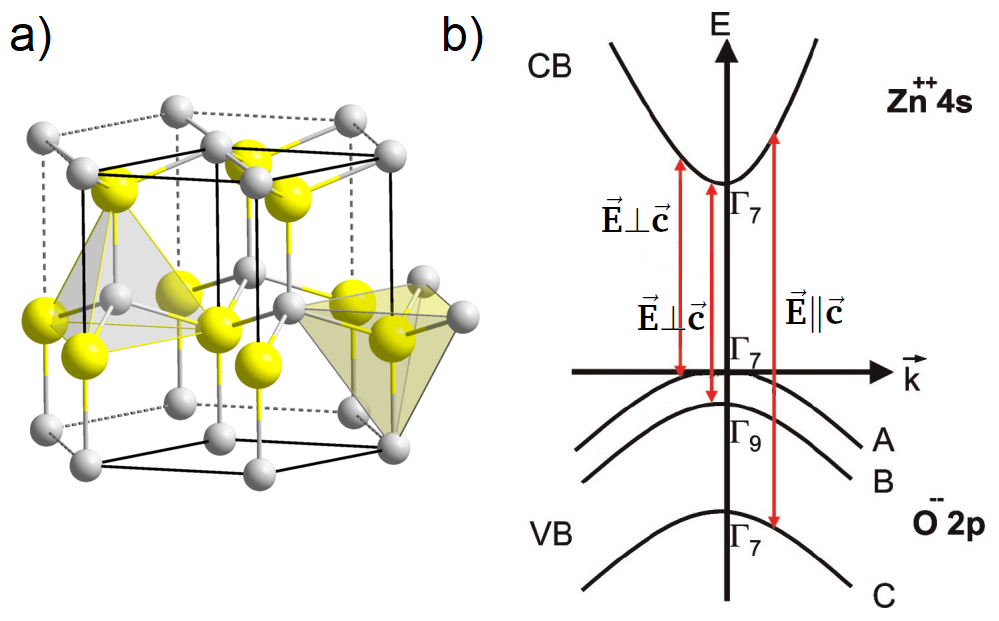
\includegraphics[width=.5\textwidth]{Bilder/Vorbetrachtung/ZnO_Str_BG}
\caption[ZnO
\section{Lumineszenz
\qquad\qquad\qquad
\mbox{Ausdehnungen}
\text{1.8}$
\textit{Mott-Wannier-Exzitonen}
\end{equation}
\cite{Mang.1995}
\mbox{Exziton}
\cite{Hopfield.1958}.
\mbox{Lichtfeld}
\mbox{Polarisation}
\mbox{statische}
\mbox{andersherum}
\cite{Klingshirn.2007}.\\
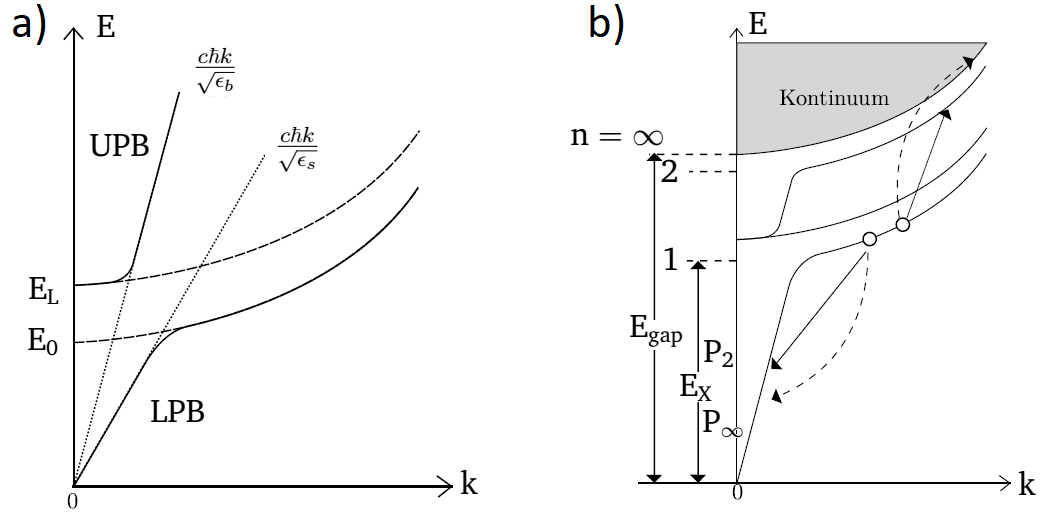
\includegraphics[width=.6\textwidth]{Bilder/Vorbetrachtung/PolScat}
\caption[Polaritonendispersion
\cite{Richters.Diss}).}
\subsection{Mehr-Exziton-Prozesse}
\textit{X-h-Streuung}).
\autoref{PolScat}).
\begin{figure}[htb]
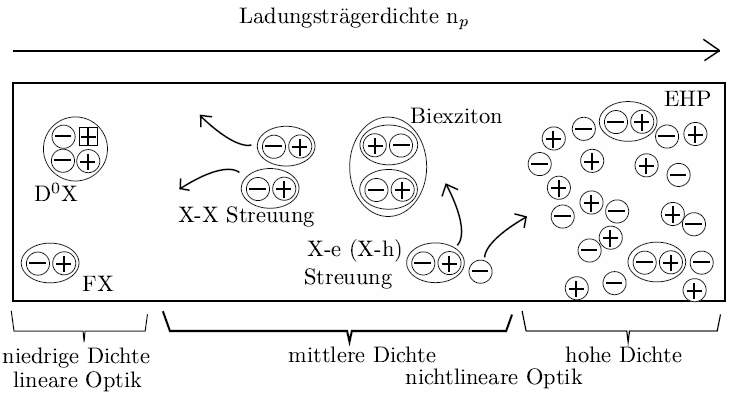
\includegraphics[width=0.7\textwidth]{Bilder/Vorbetrachtung/regimes}
\caption[
\subsection{Elektron-Loch-Plasma}
\textit{electron-hole-plasma},
\textit{Bandl
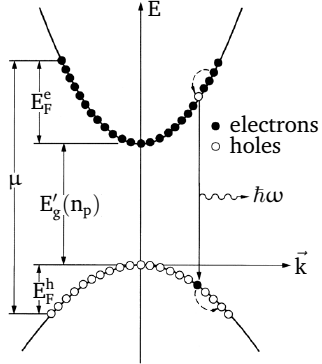
\includegraphics[width=0.3\textwidth]{Bilder/Vorbetrachtung/ehp}
\caption[Besetzung
\end{equation}
\cite{Burstein.1954}.
\subsubsection{Volumenplasmonen}
\cdot
\dot{\vec{\textbf{x}}}=-e
\sqrt{\frac{n_e\,
\subsubsection{Oberfl
\beta=\left(\frac{\omega}{c}\right)\cdot
\epsilon_2}{\epsilon_1
\textit{Besetzungsinversion}
\cite{Kneubuhl.2008}.
\cite{Kneubuhl.2008}.
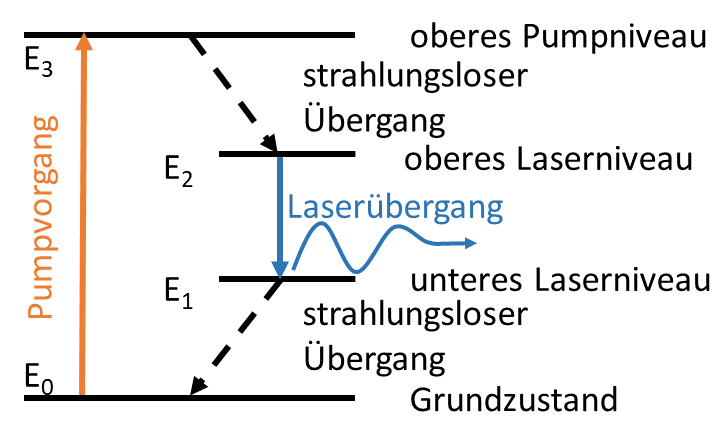
\includegraphics[width=.4\textwidth]{Bilder/Vorbetrachtung/Laseruebergang}
\caption{Laser
\end{figure}
\autoref{moden}
\textit{CDOS})
\text{0}$,
\text{7}\cdot
\cdot
\end{equation}
\cite{Maslov.2004}.
\textit{threshold})
\alpha_R(E)
\begin{figure}[b]
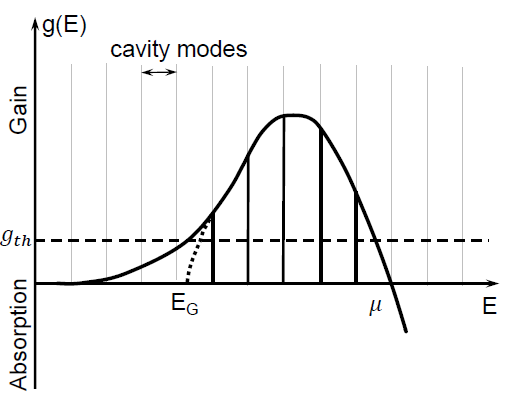
\includegraphics[width=0.35\textwidth]{Bilder/Vorbetrachtung/moden}
\caption[Verst
\end{figure}
\approx
\begin{figure}[b]
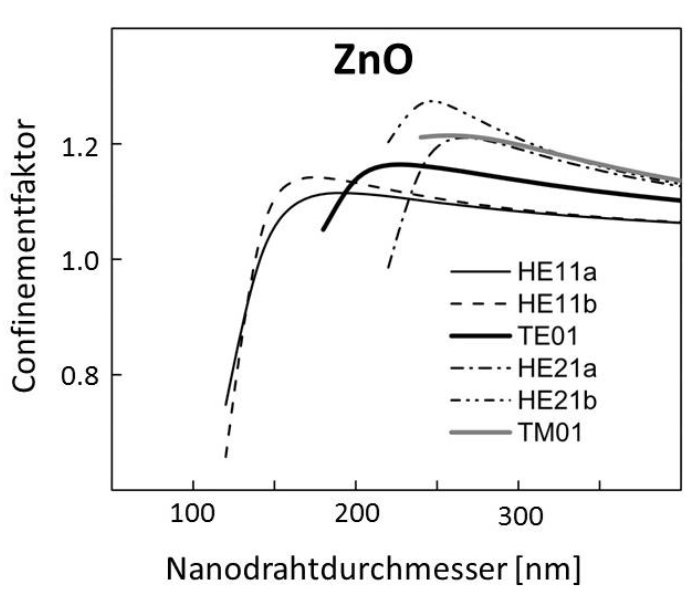
\includegraphics[width=.35\textwidth]{Bilder/Vorbetrachtung/abhd}
\caption[Abh
\label{abhd}
\subsubsection{Fabry-P
\textit{Fabry-P
\frac{1}{L}\left[\frac{\lambda^2}{2}\left(n(\lambda)-\lambda\cdot\frac{dn(\lambda)}{d\lambda}\right)^{-1}\right]
\text{
\uplambda$
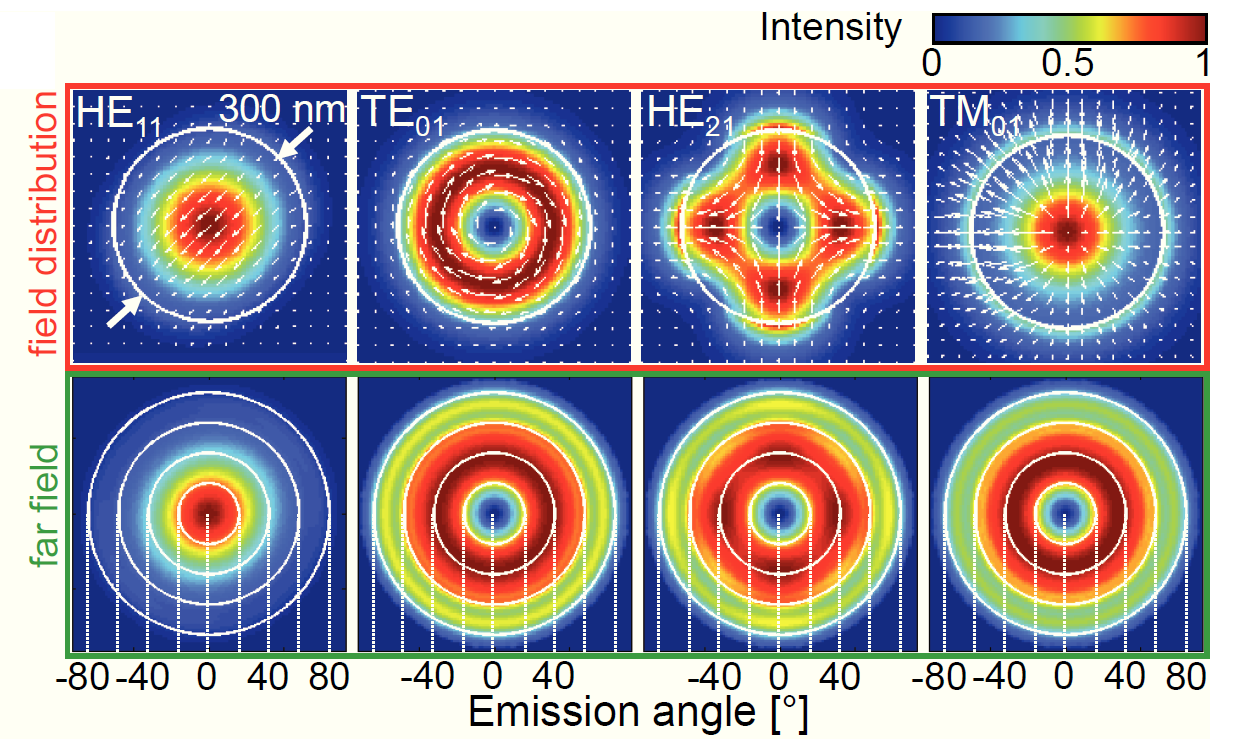
\includegraphics[width=.5\textwidth]{Bilder/Vorbetrachtung/moden2}
\caption[Feldverteilung
\cite{Roeder.Diss}).}
\subsubsection{Leistungscharakteristik}
\autoref{verst})
\begin{figure}[h]
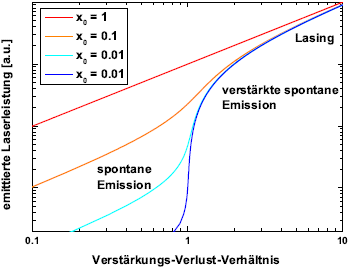
\includegraphics[width=0.4\textwidth]{Bilder/Vorbetrachtung/casperson}
\caption[Lasercharakteristik]{Doppellogarithmische
\label{casperson}
\subsection{Polarisationsrichtung
\begin{equation}
\vec{\textit{\textbf{e}}_{\textit{\textbf{r}}}}
\begin{equation}
\cdot
\begin{equation}
\frac{E_x(\vec{\textit{\textbf{z}}},t)}{E_{0,x}}\right)^2
\frac{E_y(\vec{\textit{\textbf{z}}},t)}{E_{0,y}}
\end{equation}
\frac{\uppi}{\text{2}}$
\mbox{Amplitudenverh
\label{IntroStokesParams}
\begin{equation}
\end{equation}
\cite{Stokes.1851}.
\end{equation}
\begin{equation}
\right)
\right)_{UP}
\right)_{P}
\text{mit
\section{Magnetismus
\cite{Gross.2014}.
\vec{\textbf{j}}_{\textbf{i}}$.
\vec{\textbf{j}}_{\textbf{i}}$
\vec{\textbf{l}}_{\textbf{i}}$
\vec{\textbf{s}}_{\textbf{i}}$,
\text{-(l-1),
\subsection{Larmorpr
\vec{\textit{\textbf{B}}}
\end{equation}
\vec{\textbf{$\omega$}}_{\textit{\textit{\textbf{L}}}}
\vec{\textit{\textbf{J}}}
\vec{\textit{\textbf{B}}}.
\textit{anormaler
\textit{normalen
\subsection{Auswahlregeln
\text{1}$
\begin{equation}
\begin{figure}[h]
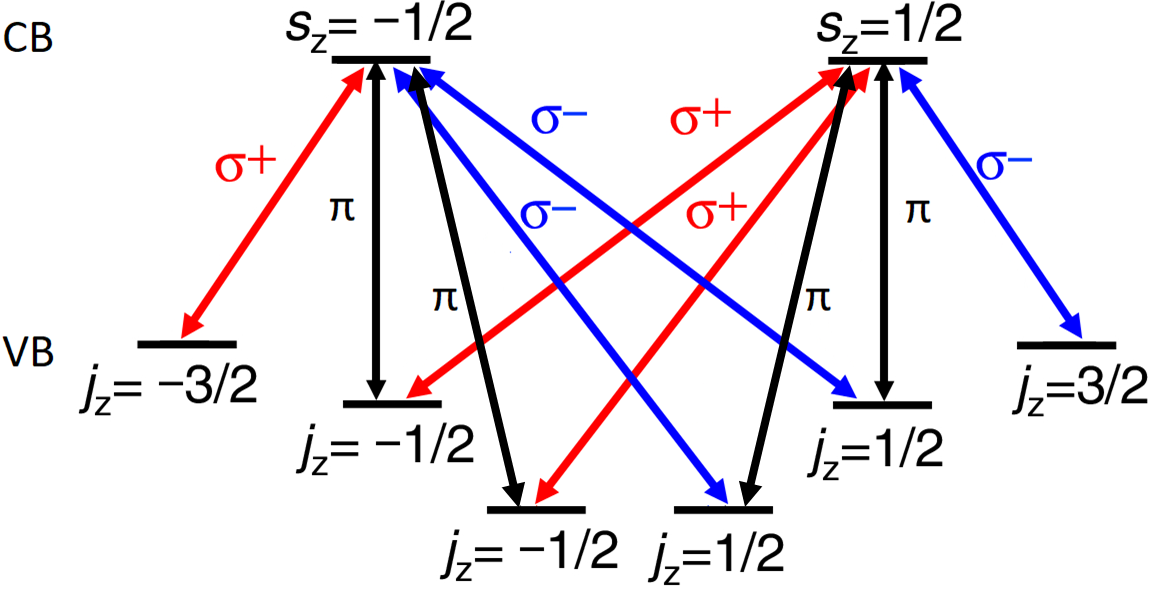
\includegraphics[width=.5\textwidth]{Bilder/Vorbetrachtung/ausw}
\caption[Auswahlregeln]{M
\end{figure}
\frac{\tau}{\tau_{SR}}}
\cite{Dyakonov.2008}.
\subsubsection{Spinrelaxationszeit
\begin{equation}
\text{
\subsubsection{Spindekoh
\end{equation}
\begin{equation}
\subsubsection{Der
\Psi_{\vec{\textbf{k}},n,\uparrow}(\vec{\textbf{r}})=\left(
\vec{\textbf{k}}\cdot
\Psi_{\vec{\textbf{k}},n,\downarrow}(\vec{\textbf{r}})=\left(
\vec{\textbf{k}}\cdot
\mid\text{a}_{\vec{\textbf{k}},\text{n}}\mid$).
\textit{Spinflip}.
\tau_{SR}
\begin{equation}
\left(\frac{\Delta_{SO}}{E_g
\left(\frac{E_k}{E_g}\right)^2
\textit{DPM})
\text{
\,\Omega
\Upomega$.
\begin{equation}
\end{equation}
\frac{1}{\uptau_{SR}}
\gg
\cite{Zutic.2004}.
\label{DPM_Mag}
\upomega_\text{L}
\begin{equation}
\tau_{c})^2}=\frac{\Omega^2
\end{equation}
\subsubsection{Der
\cite{Hanle.1924}
\mbox{Materialsystem},
\mbox{Polarisationsgrad}
\vec{\textbf{$\omega_L$}}\times
\vec{\textbf{S}}-\frac{\vec{\textbf{S}}}{\tau_{SR}}-
\frac{\vec{\textbf{S}}-\vec{\textbf{$S_0$}}}{\tau}
\subsection{Nanodrahtsynthese
\textit{HTJ})
\cite{Geburt.Diss}.
\end{table}
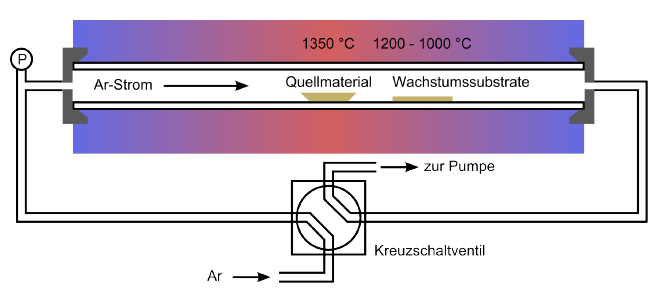
\includegraphics[width=.75\textwidth]{Bilder/Methodik/htj}
\caption[Schematischer
\subsection{Imprint}
\cite{Epstein.2002}.
\autoref{magres})
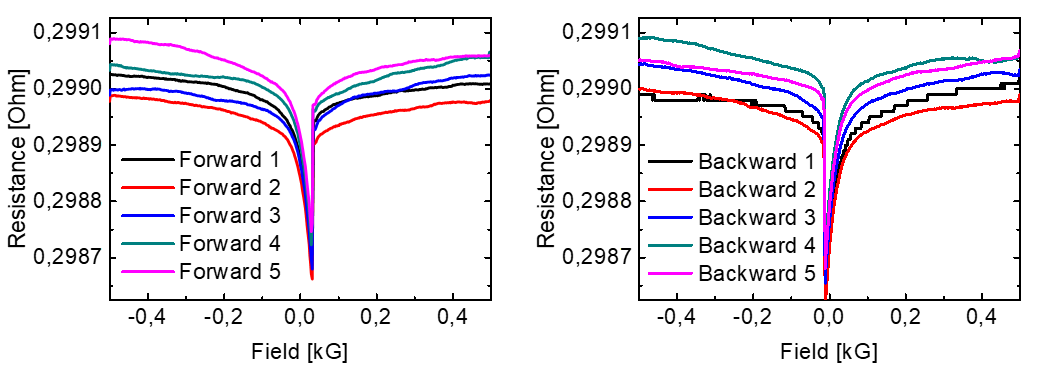
\includegraphics[width=.85\textwidth]{Bilder/Methodik/magnres}
\caption[Magnetowiderstandsmessung
\cdot
\begin{tabular}{lllll}
\end{tabular}
\begin{figure}[h]
\includegraphics[width=1\textwidth]{Bilder/Methodik/Sim_mag_komplett}
\caption[Simulation
\subsection{Mikro-Photolumineszenz
\autoref{AufbauPL}).
\textit{Pellin-Broca-Prisma}
\\
\autoref{Justage}).
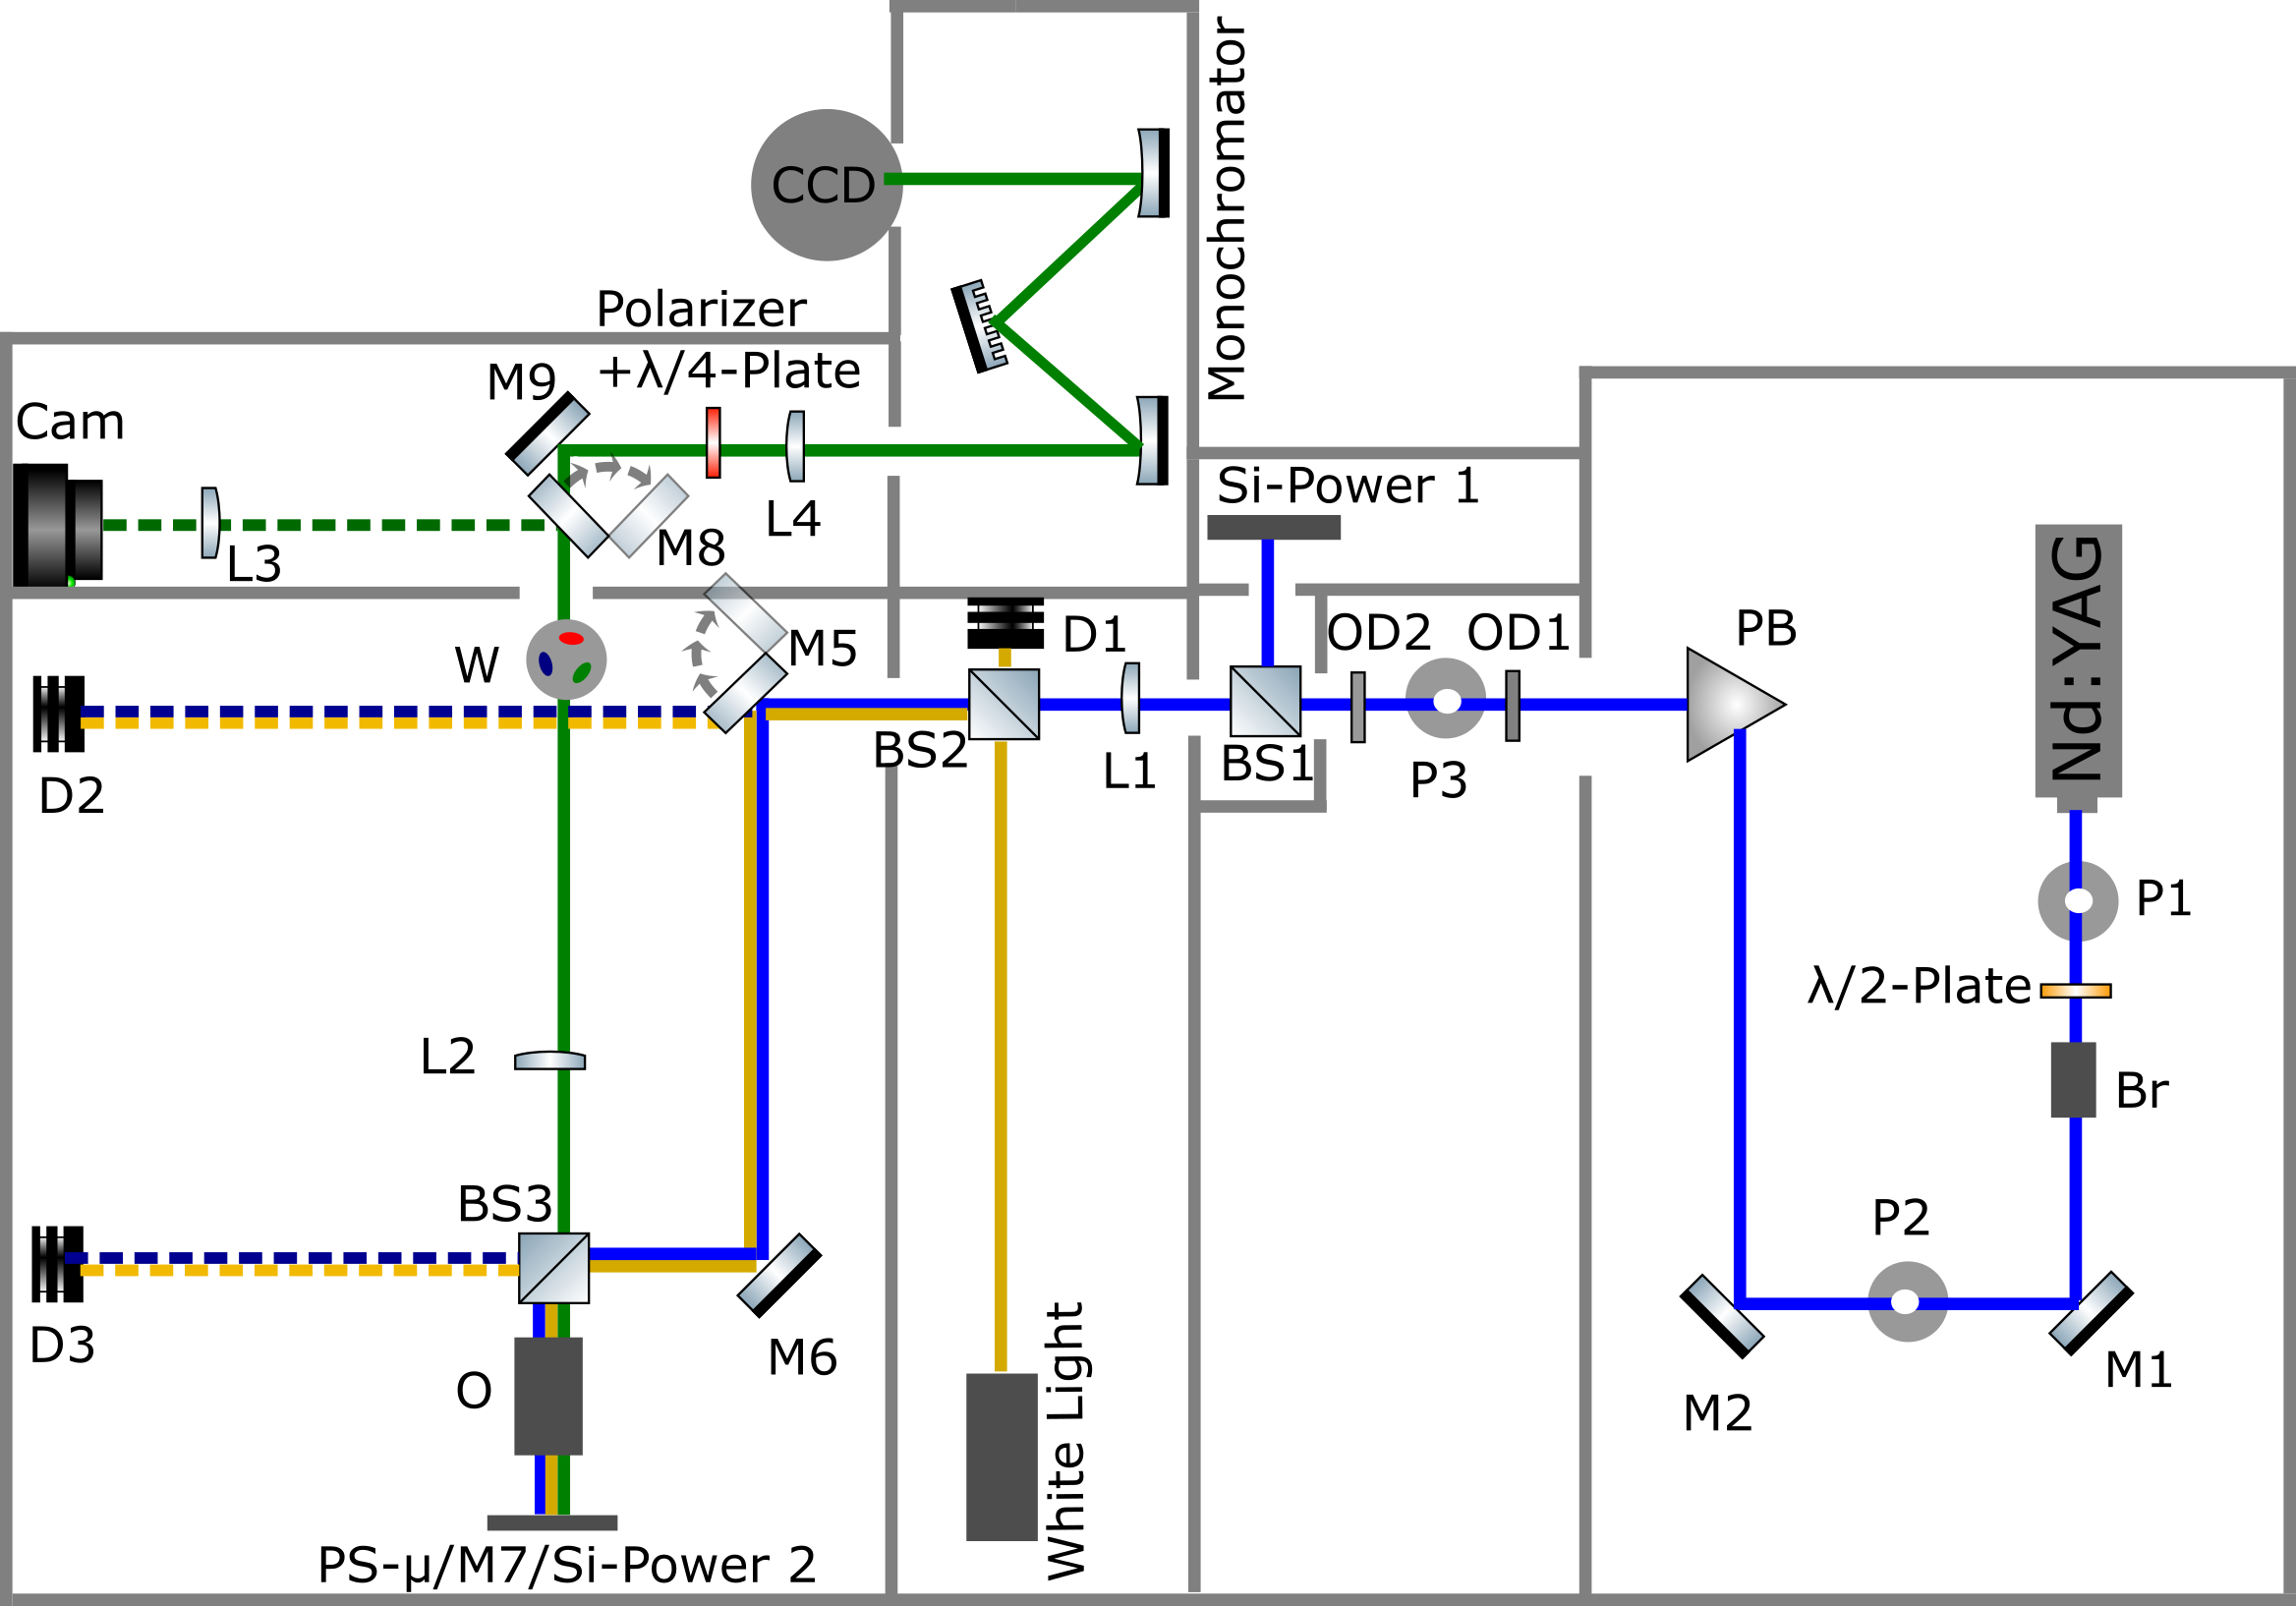
\includegraphics[width=1\textwidth]{Bilder/methodik/opt_aufb}
\cite{lib}.
\subsubsection{Kalibrierung
\text{
\autoref{laserspot}
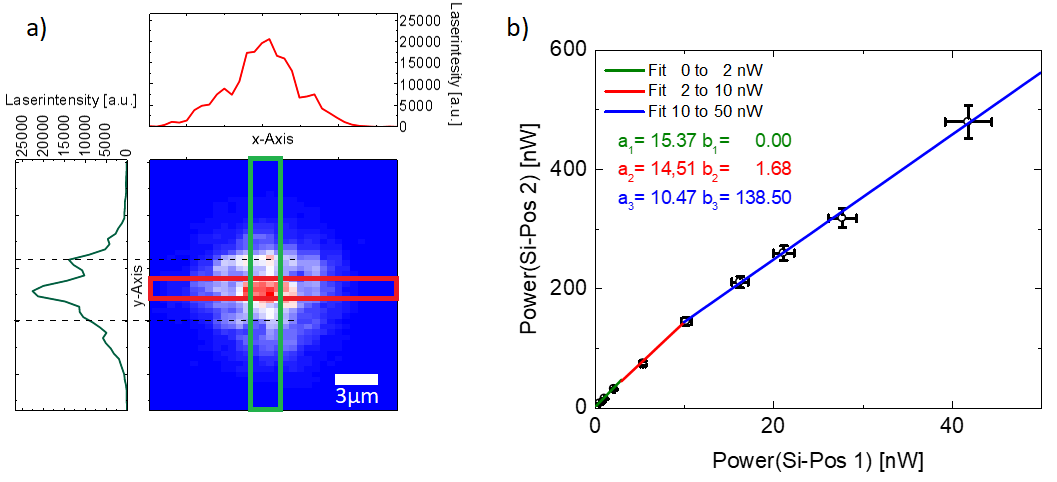
\includegraphics[width=1\textwidth]{Bilder/Methodik/spotsize}
\caption{Darstellung
\subsubsection{Erstellung
\subsubsection{Fourier
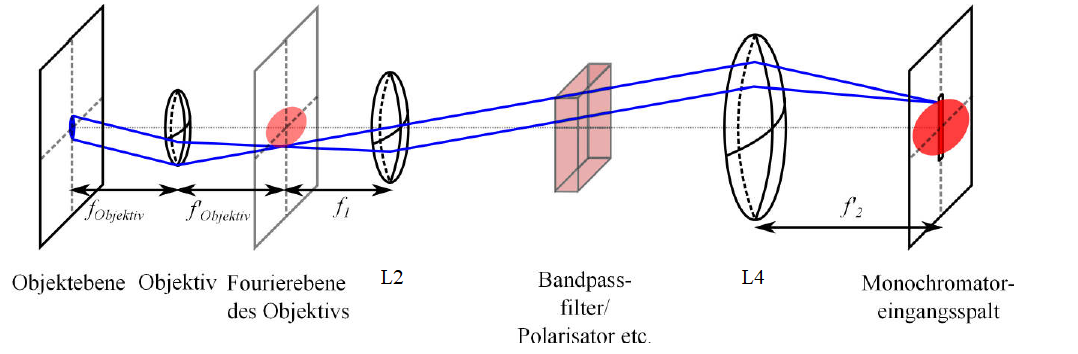
\includegraphics[width=1\textwidth]{Bilder/Methodik/fourier}
\caption[Impulsraumabbildung]{Strahlengang
\cite{Master.Michalsky}).}
\textit{back
\cite{Riediger.Master}
\uptheta_{max}=arcsin\left(n(\uplambda)\cdot
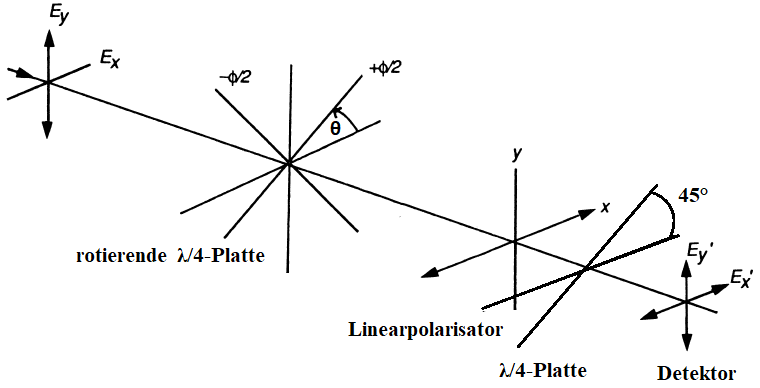
\includegraphics[width=.8\textwidth]{Bilder/Methodik/stokesaufbau}
\caption{Aufbau
\cite{Goldstein.2003}).}
\cite{Schaefer.2007}
\end{equation}
\begin{equation}
\cite{Goldstein.2003}.
\text{47.4}^\circ
\label{StokesGl7}
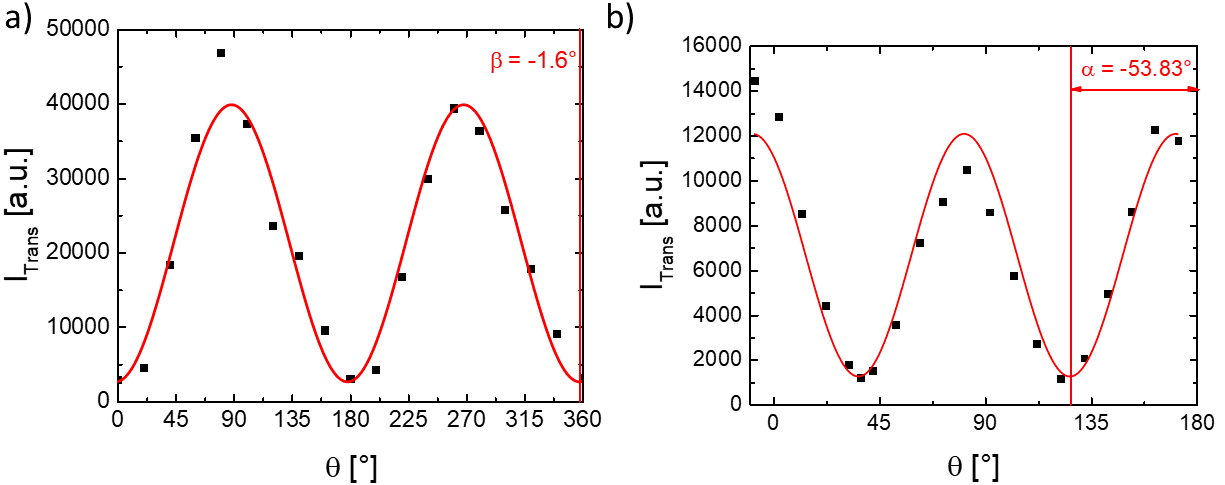
\includegraphics[width=1\textwidth]{Bilder/Methodik/OptElemente}
\caption{Darstellung
\frac{1
\frac{2}{1-cos(\delta)}\,\left[
\,
\textit{SEM})
\autoref{S0_reconstruct_SiO2_S1_6}
\autoref{horvert_reconstruct_SiO2_S1_6}
\centering
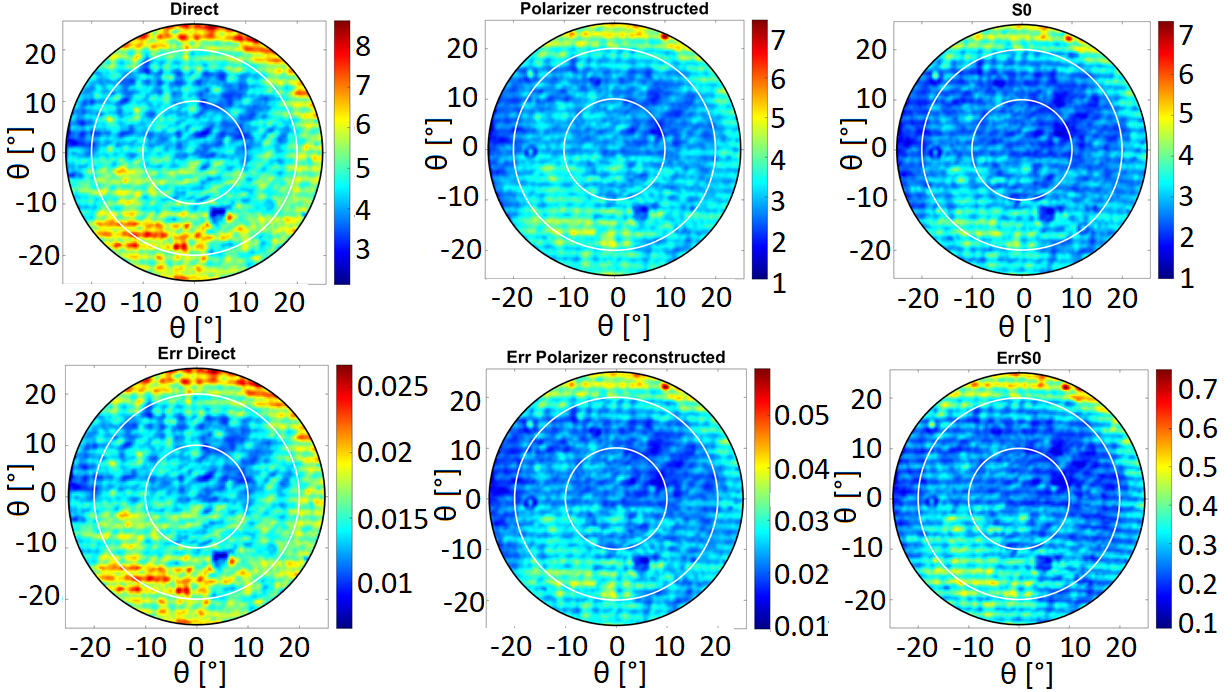
\includegraphics[width=.75\textwidth]{Bilder/Methodik/S0_reconstruct_SiO2_S1_6}
\caption{Obere
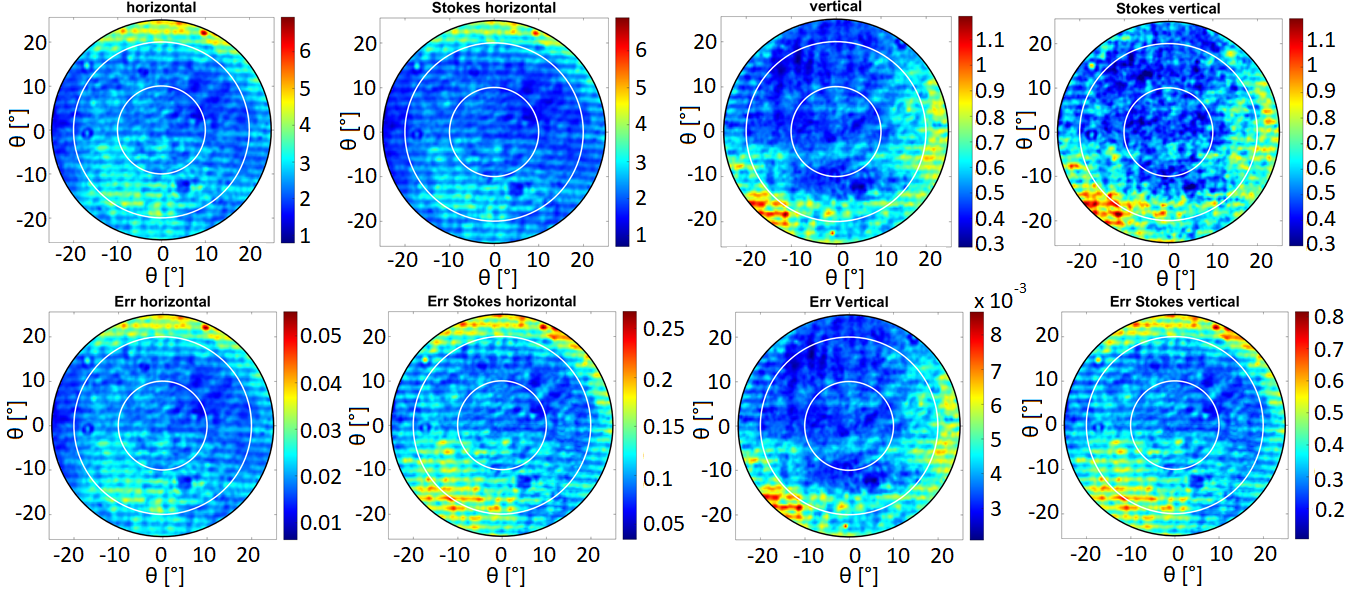
\includegraphics[width=1\textwidth]{Bilder/Methodik/horvert_reconstruct_SiO2_S1_6}
\caption{Obere
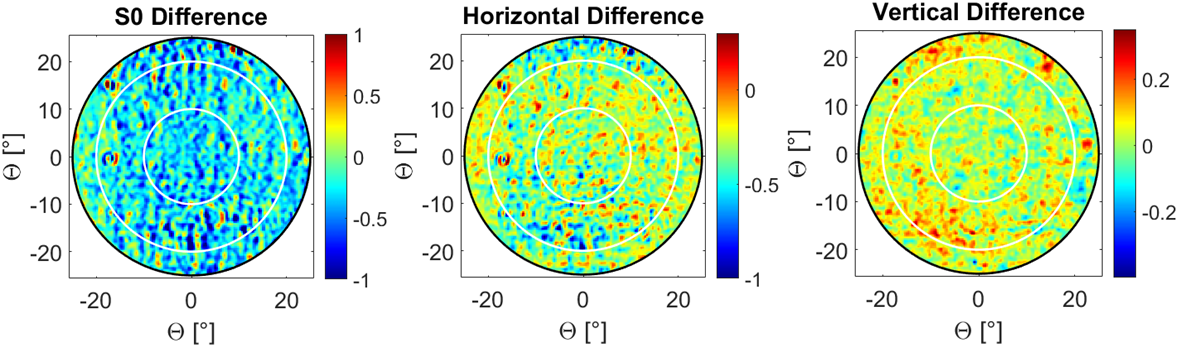
\includegraphics[width=.75\textwidth]{Bilder/Methodik/Diff_reconstruct_SiO2_S1_6}
\caption{Darstellung
\autoref{S0_reconstruct_SiO2_S1_6}
\label{Diff_SiO2_S1_6}
\autoref{SEM_SiO2_S1_6}).
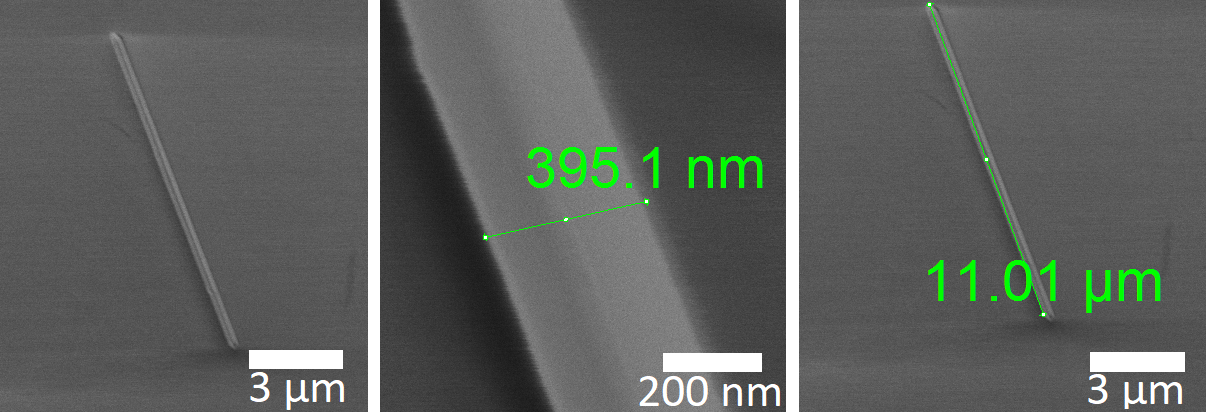
\includegraphics[width=.6\textwidth]{Bilder/SiO2/SEM_SiO2_S1_6}
\caption{REM-Bilder
\text{11
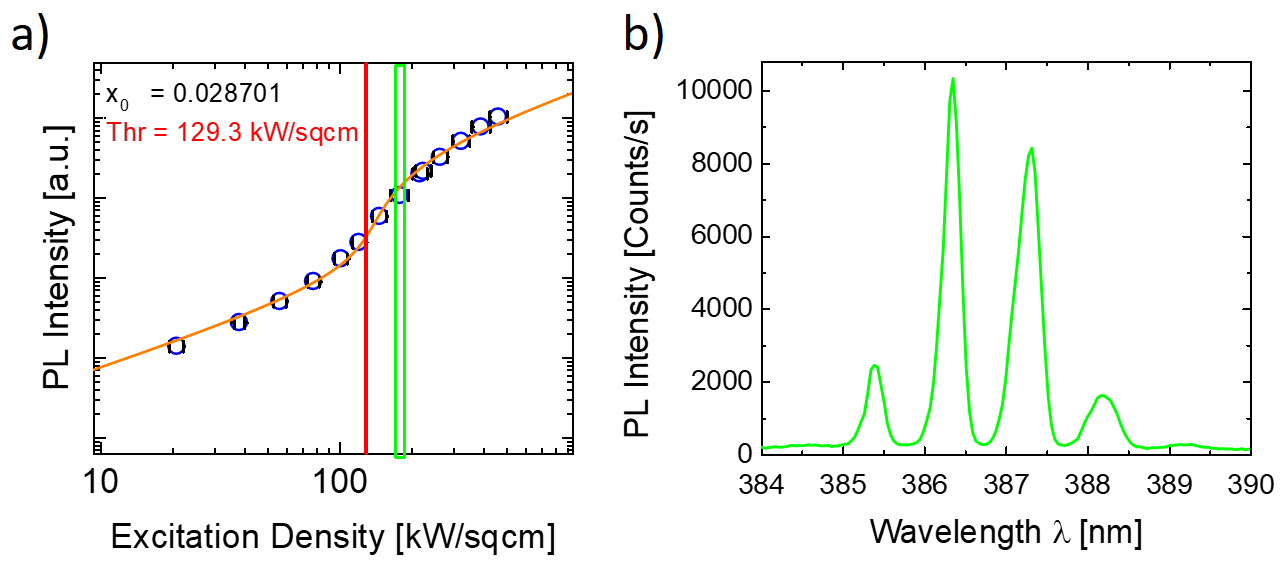
\includegraphics[width=.6\textwidth]{Bilder/SiO2/Cas_SiO2_S1_6}
\autoref{SEM_SiO2_S1_6}
\frac{dn}{d\lambda}=\frac{\left(n
\Delta\lambda}\right)}{\lambda}
\label{Disp}
\cite{Zimmler.2010}
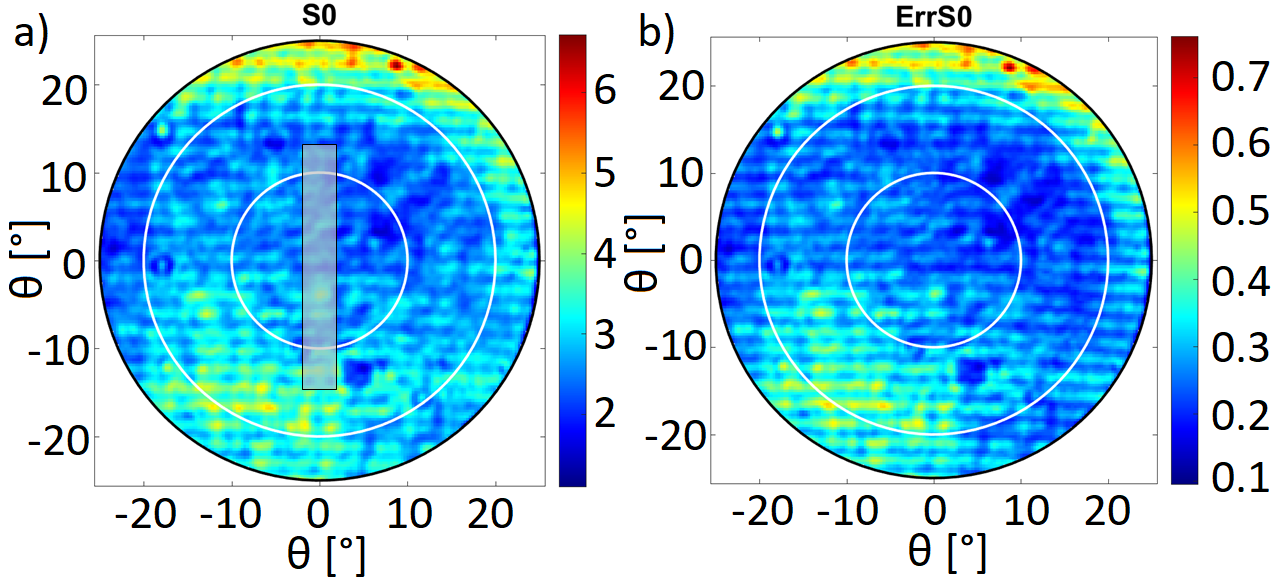
\includegraphics[width=.55\textwidth]{Bilder/SiO2/S0_S1_Si02_6}
\autoref{SEM_SiO2_S1_6}
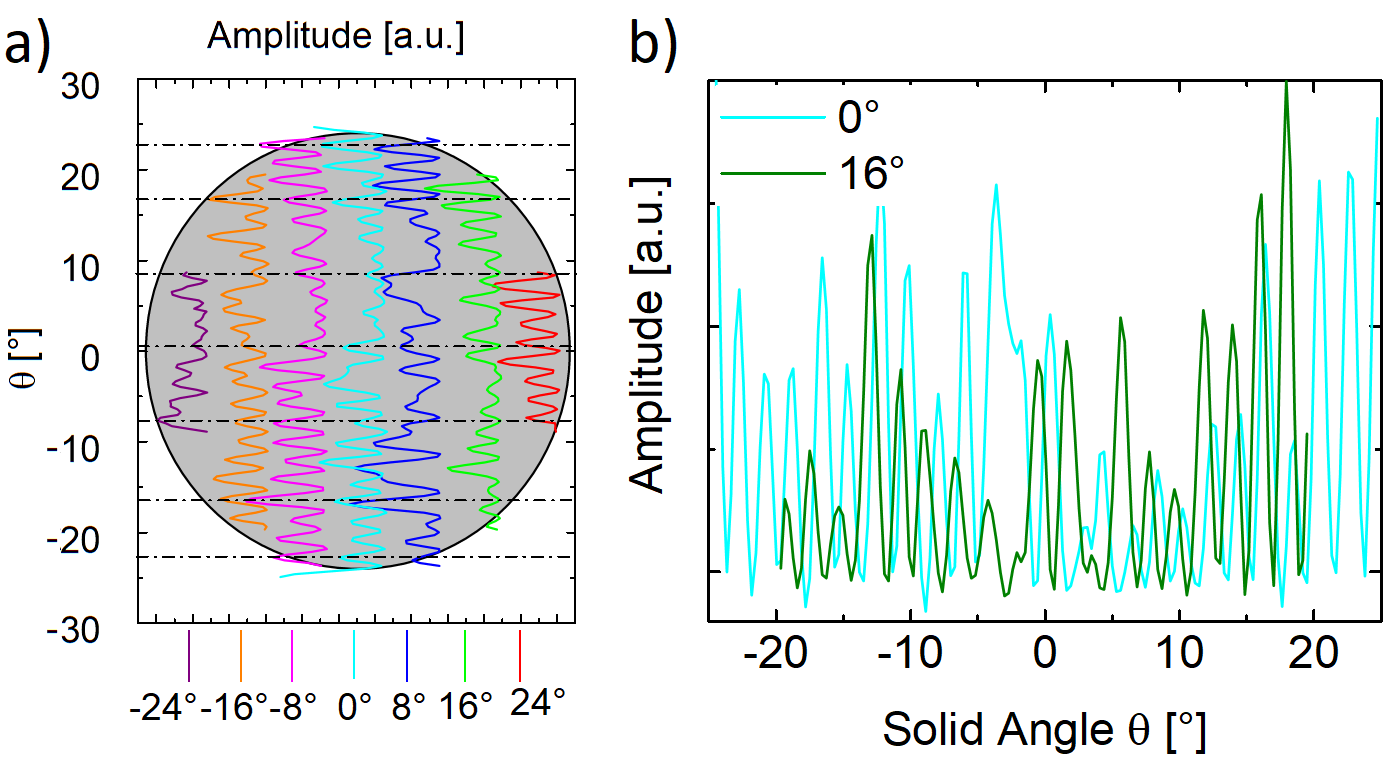
\includegraphics[width=.7\textwidth]{Bilder/SiO2/Vert_Linescan_SiO2_S1_6}
\caption{Darstellung
\ldots
\autoref{S0_S1_Si02_6}
\end{equation}
\text{386.7}$
\autoref{SEM_SiO2_S1_6})
\text{m}$
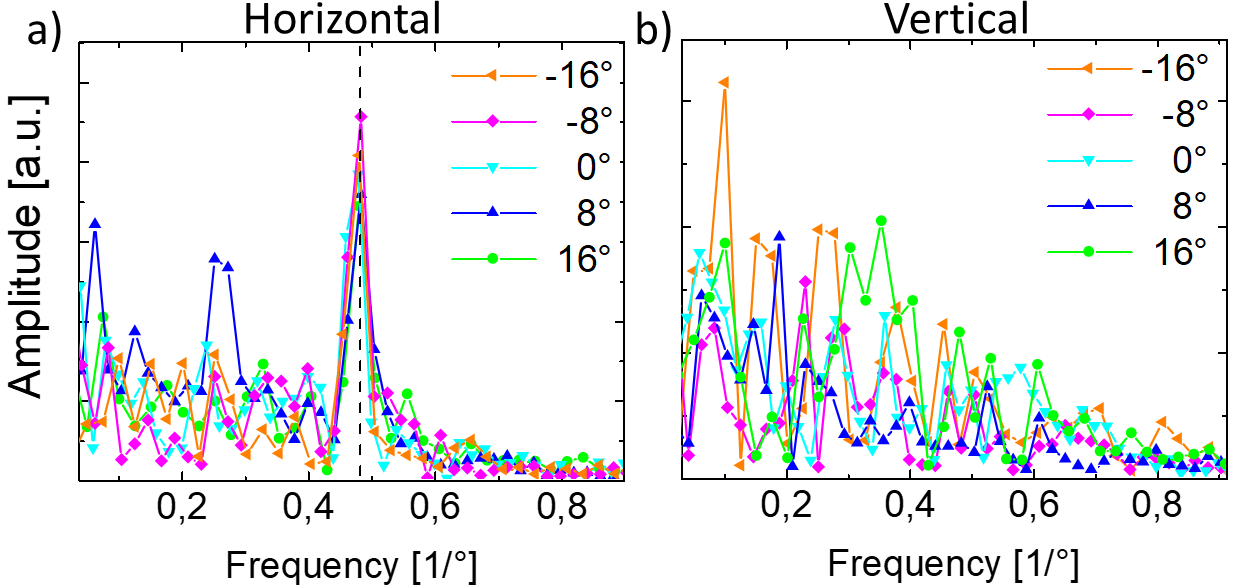
\includegraphics[width=.66\textwidth]{Bilder/SiO2/FFT_Linescan_SiO2_S1_6}
\caption{Fouriertransformation
\autoref{Vert_Linescan_SiO2_S1_6},
\autoref{S0_Spec_S1_Si02_6}).
\autoref{Rec_Spec_S1_Si02_6}
\autoref{Cas_SiO2_S1_6}
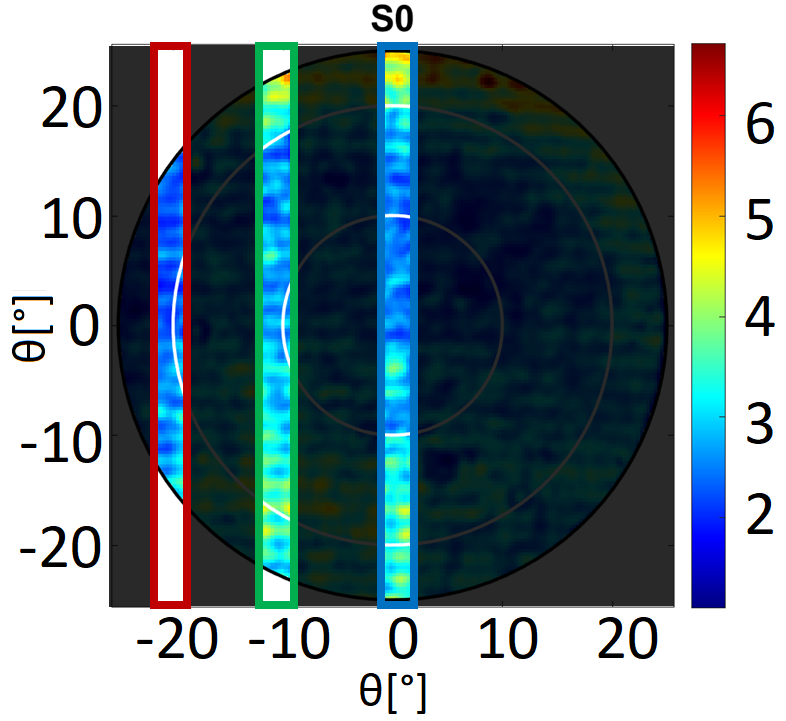
\includegraphics[width=.33\textwidth]{Bilder/SiO2/S0_Spec_1_S1_Si02_6}
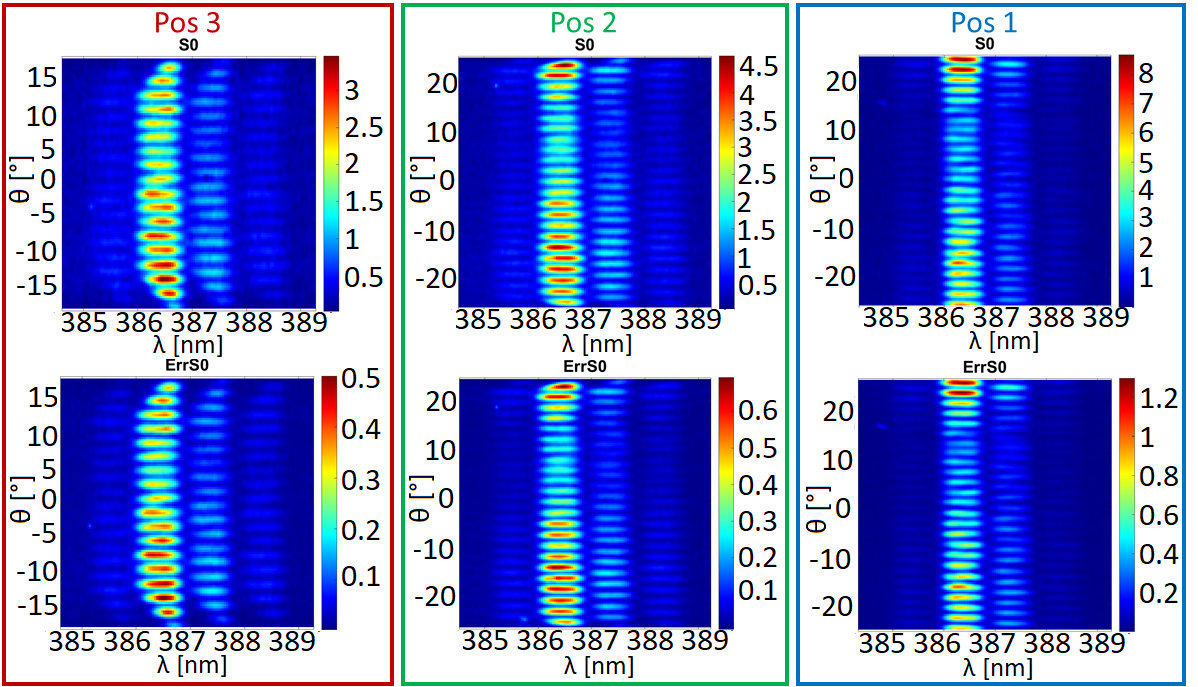
\includegraphics[width=.75\textwidth]{Bilder/SiO2/S0_Spec_S1_Si02_6}
\caption{Darstellung
\end{figure}\begin{table}[h]
\caption{Nummerierung
\label{ModenNum}
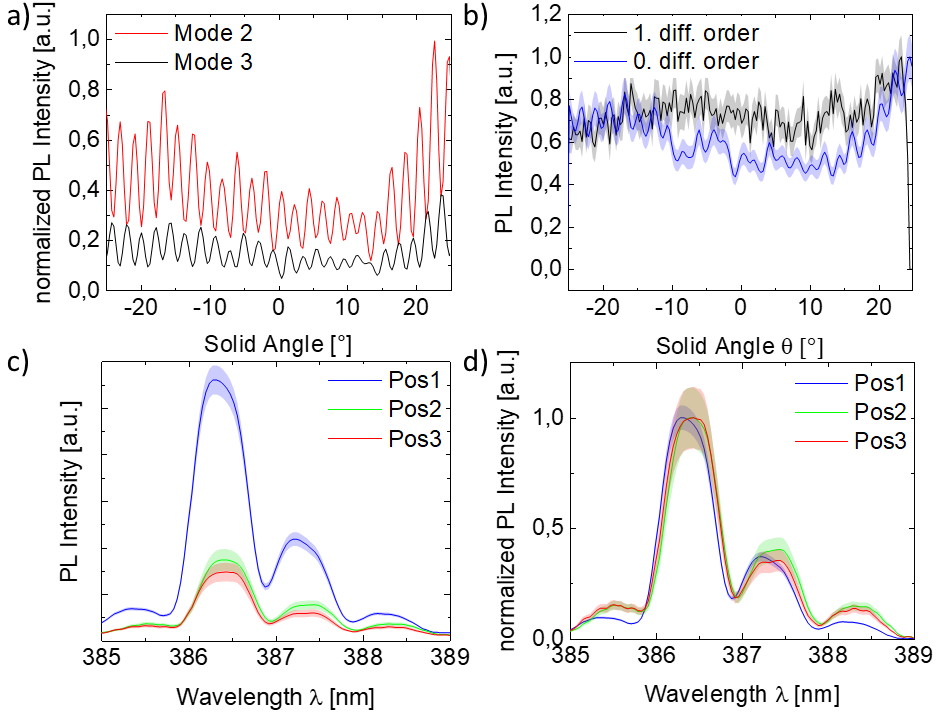
\includegraphics[width=.6\textwidth]{Bilder/SiO2/Rec_Spec_S1_Si02_6}
\subsection{Polarisationseigenschaften
\label{PolGradSiO2}
\autoref{SEM_SiO2_S1_6}
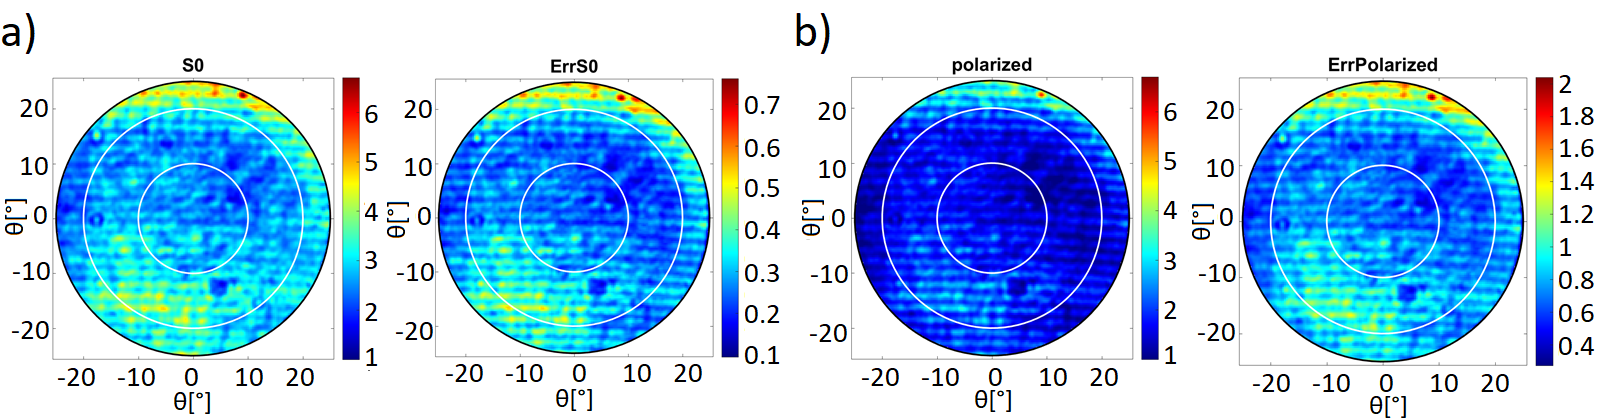
\includegraphics[width=1\textwidth]{Bilder/SiO2/Pol_SiO2_S1_6}
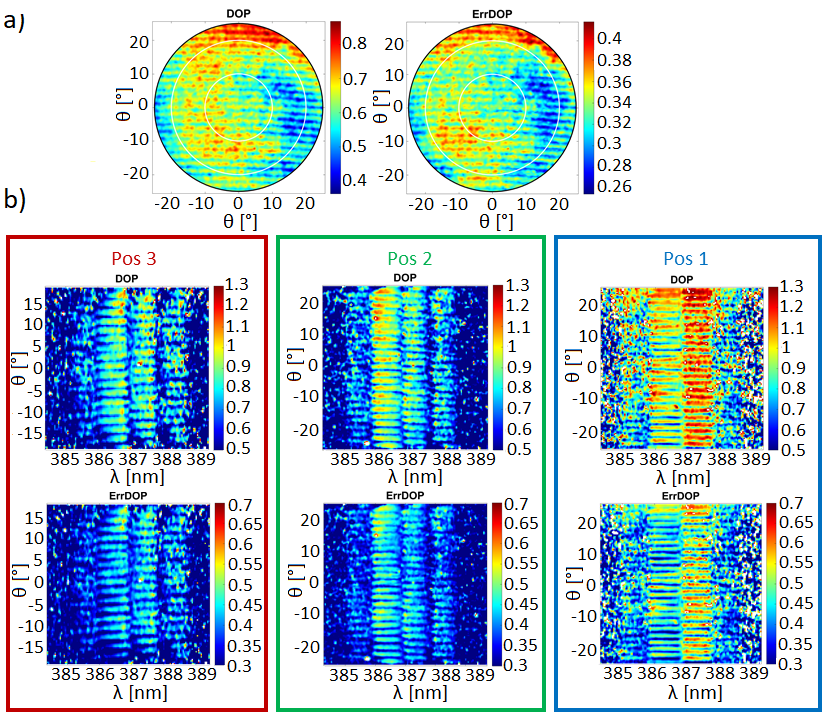
\includegraphics[width=0.75\textwidth]{Bilder/SiO2/DOP_SiO2_S1_6}
\caption{Darstellung
\autoref{DOP_SiO2_S1_6}
\autoref{compSpec_2_DOP})
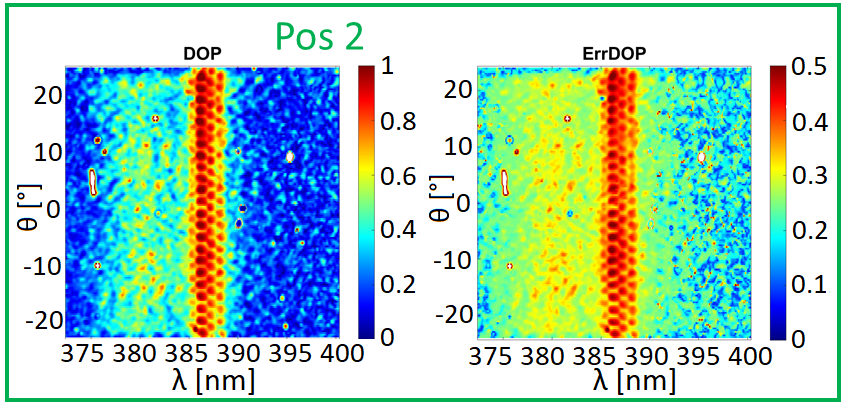
\includegraphics[width=.55\textwidth]{Bilder/SiO2/compSpec_2_DOP}
\caption{Darstellung
\end{figure}Es
\bot
\autoref{Rauschen})
\autoref{S0_S1_Si02_6}),
\subsubsection{Stokes-Parameter
\autoref{IntroStokesParams}).
\centering
\caption{Obere
\autoref{SEM_SiO2_S1_6}
\autoref{StokesP_S1_SiO2_6}
\autoref{StokesP_S1_SiO2_6}
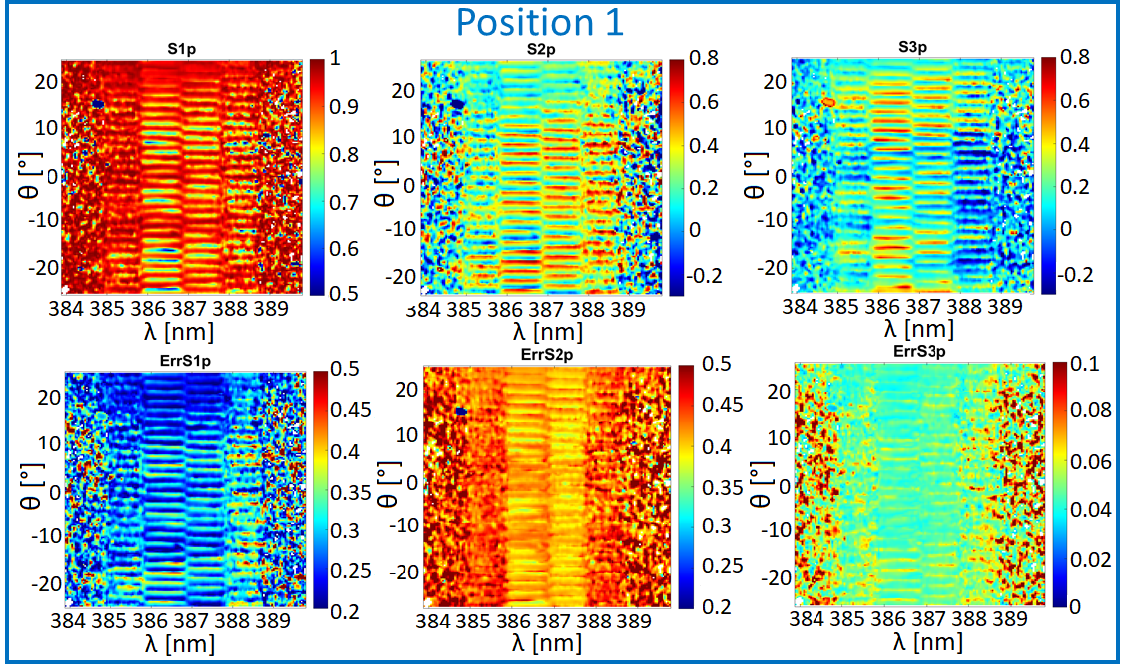
\includegraphics[width=0.66\textwidth]{Bilder/SiO2/SpecP1_StokesP_S1_Si02_6}
\caption{Obere
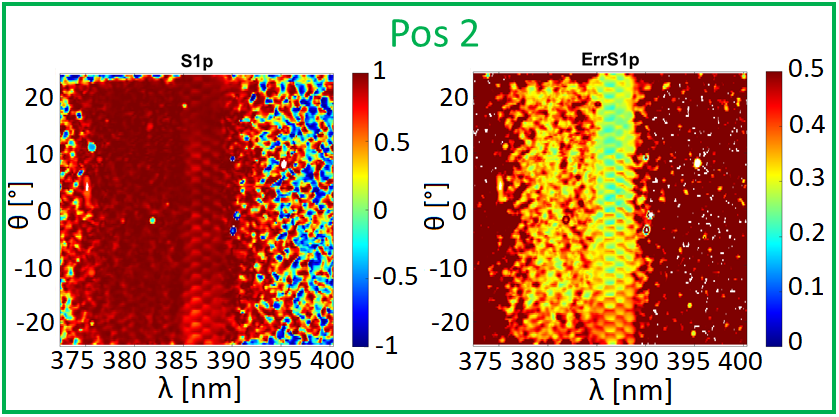
\includegraphics[width=0.5\textwidth]{Bilder/SiO2/compSpec_2_S1p}
\caption{Darstellung
\label{compSpec_2_S1p}
\textit{degree
\autoref{DOLP_S1_SiO2_6}).
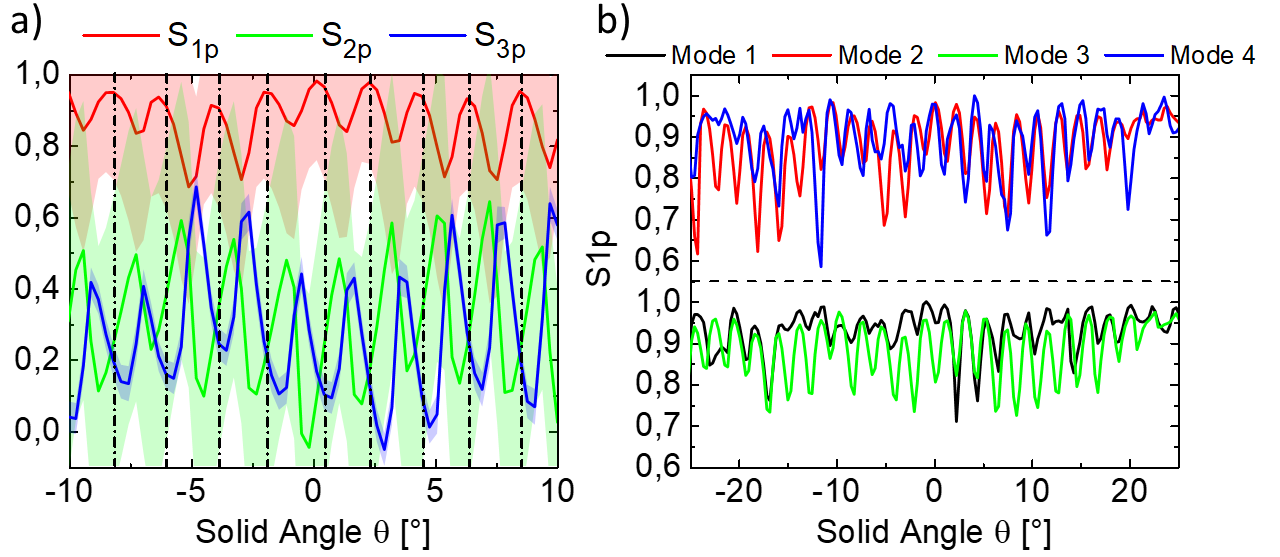
\includegraphics[width=.66\textwidth]{Bilder/SiO2/SpecP1_StokesP_Line_S1_Si02_6}
\caption{a)
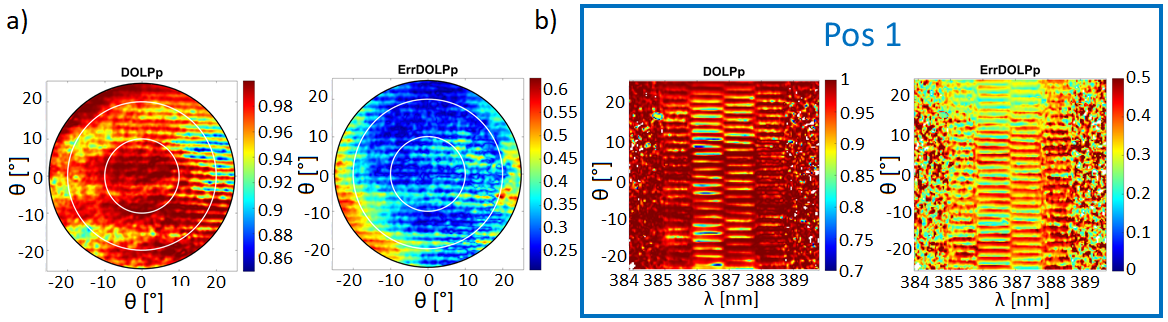
\includegraphics[width=1\textwidth]{Bilder/SiO2/DOLP_SiO2_S1_6}
\label{DOLP_S1_SiO2_6}
\mbox{(engl.
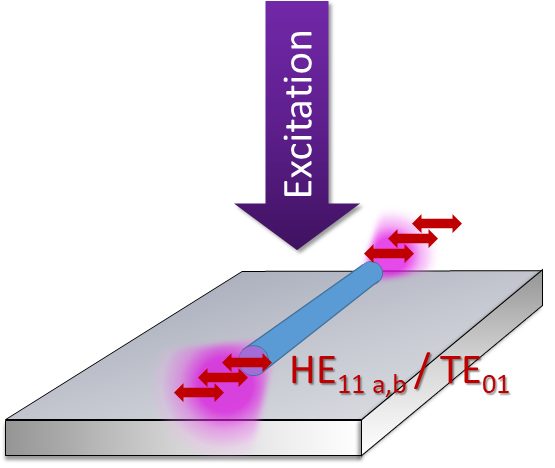
\includegraphics[width=.35\textwidth]{Bilder/SiO2/PolPic}
\autoref{S0_S1_Si02_6}),
\section{ZnO-Nanodr
\includegraphics[width=0.7\textwidth]{Bilder/MgO/SEM_MgO_S1_1_3}
\caption{REM-Bilder
\centering
\caption{Integrierte
\autoref{SEM_MgO_S1_1_3}.}
\autoref{CasFit_S1_MgO_13}
\autoref{SEM_SiO2_S1_6},
\autoref{CasFit_S1_MgO_13}
\autoref{CasFit_S1_MgO_13}
\cite{Sidiropoulos.2014}.
\centering
\caption{Vergleich
\autoref{CasFit_S1_MgO_13}
\frac{dn}{d\lambda}\,
\end{equation}
\cite{Wille.2016}.
\subsubsection{Drahtkombinationen}
\autoref{SEM_MgO_S2_0}),
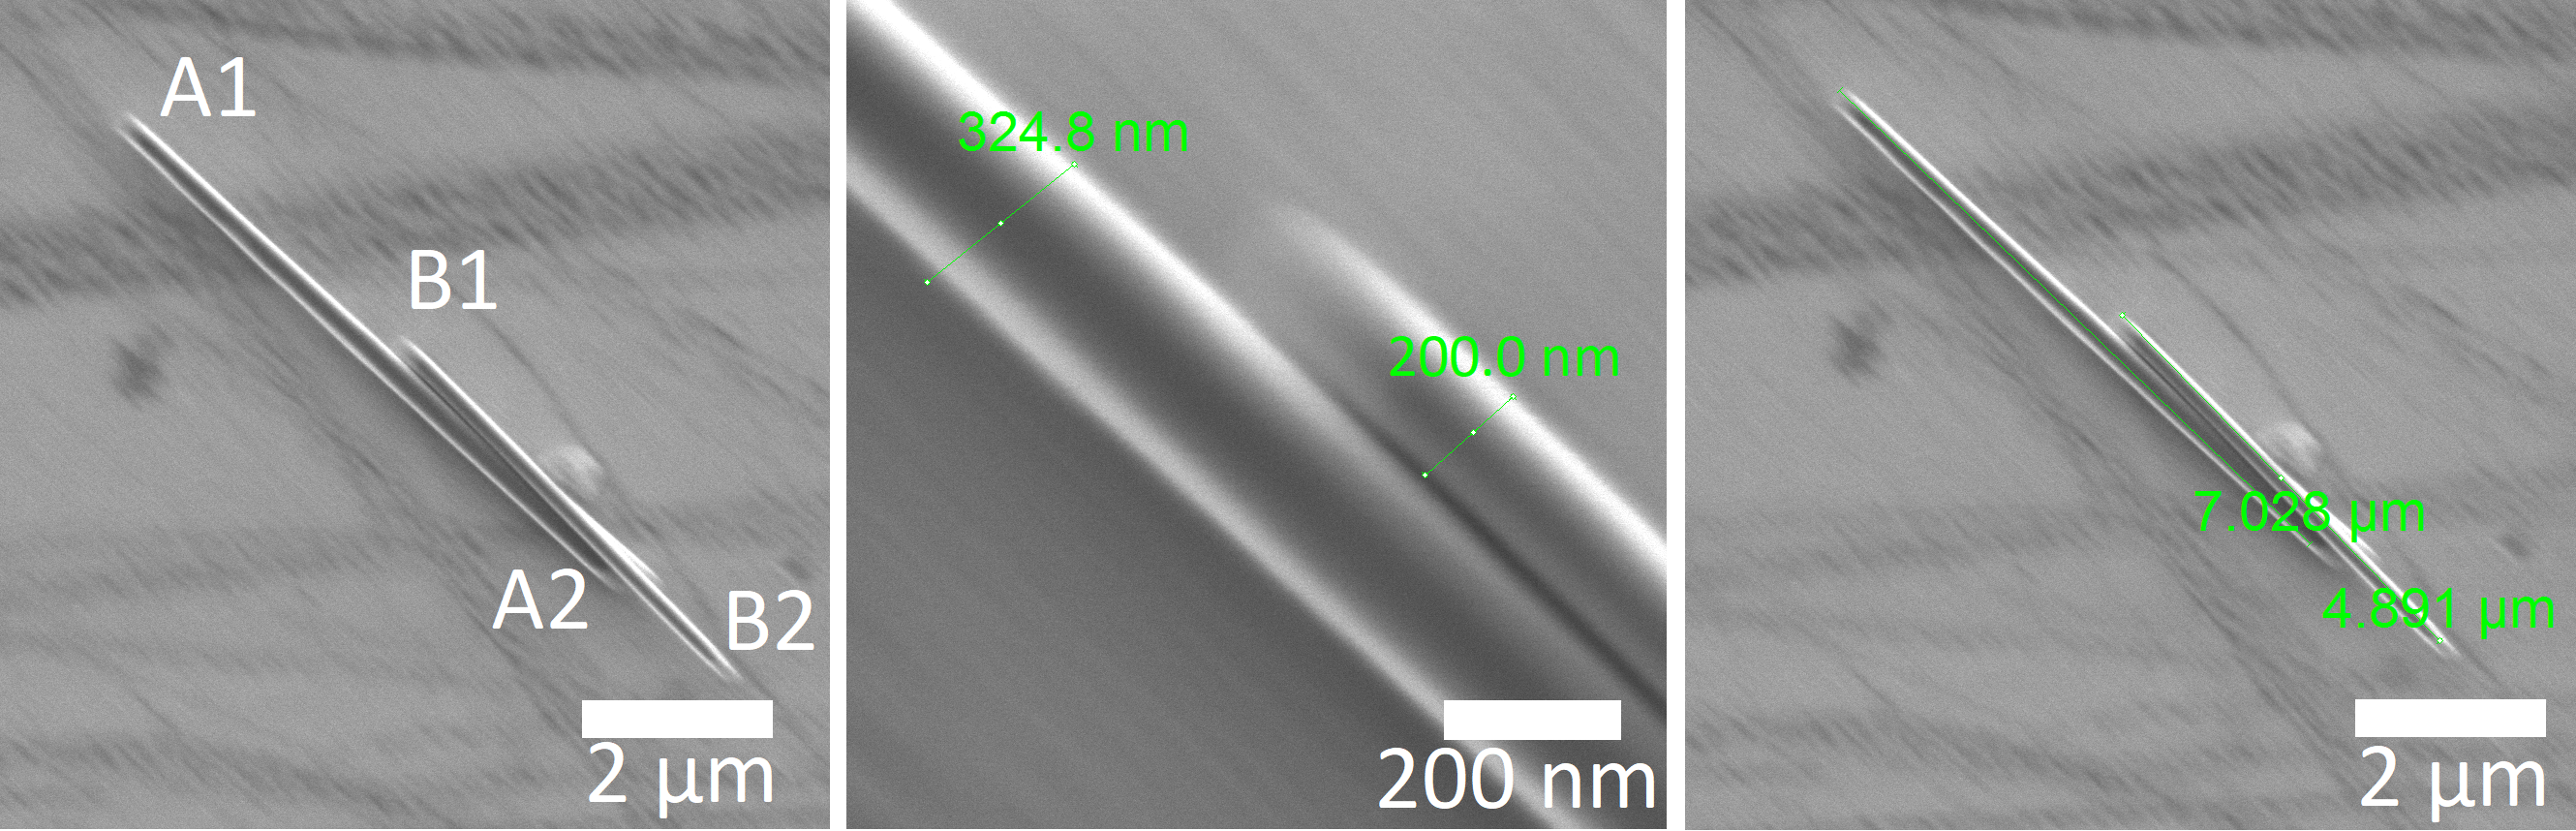
\includegraphics[width=0.7\textwidth]{Bilder/MgO/SEM_MgO_S2_0}
\approx
\text{325
\text{8.95
\text{525
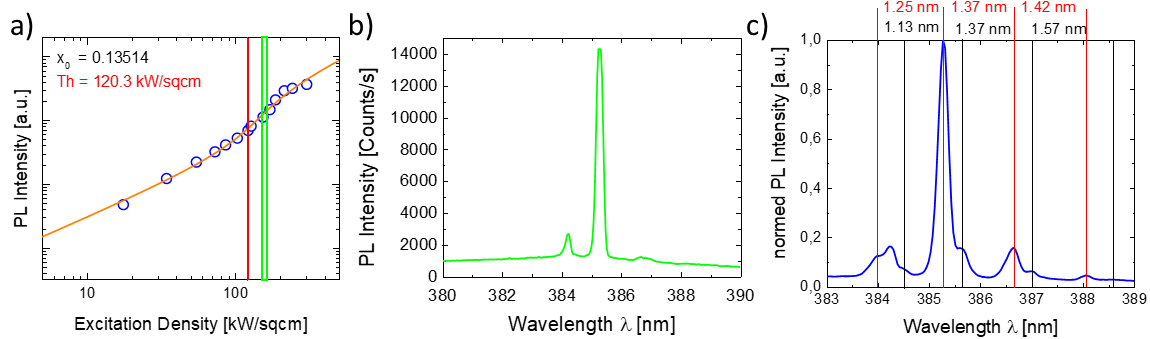
\includegraphics[width=1\textwidth]{Bilder/MgO/Cas_MgO_S2_0}
\autoref{SEM_MgO_S2_0}
\label{Cas_MgO_S2_0}
\autoref{Cas_MgO_S2_0}
\begin{tabular}{llllll}
\caption{Abst
\label{YoungDist}
\autoref{ResBed}
\left[\frac{1}{2}\,
\left(n(\lambda)-\lambda\cdot\frac{dn(\lambda)}{d\lambda}\right)^{-1}\right]
\text{
\autoref{Disp}
\subsection{Fourierabbildung
\autoref{S0_S2_MgO_0}
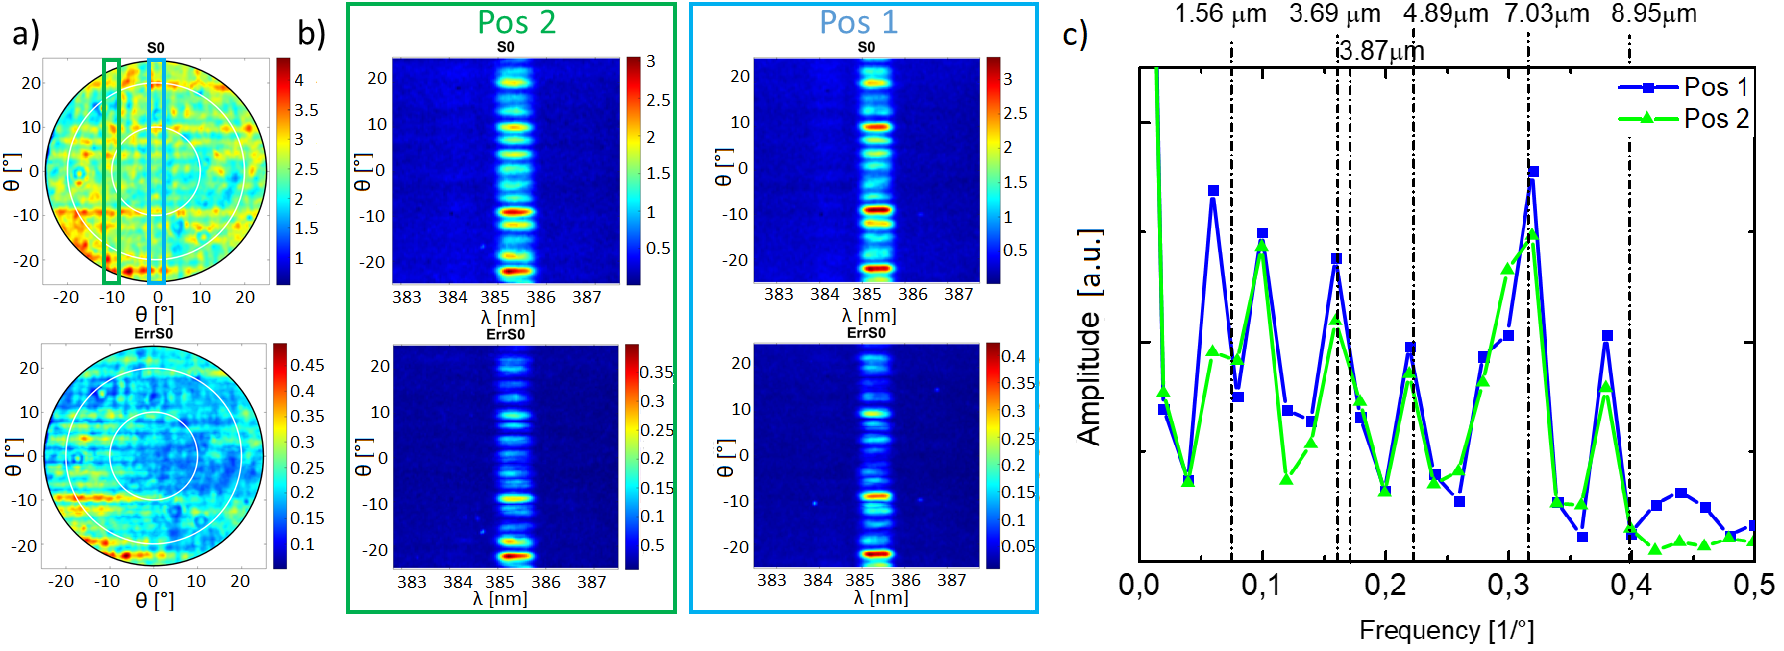
\includegraphics[width=1\textwidth]{Bilder/MgO/S0_S2_MgO_0}
\autoref{SEM_SiO2_S1_6}
\label{S0_S2_MgO_0}
\begin{equation}
\subsection{Polarisationseigenschaften
\autoref{DOP_MgO_S2_0}
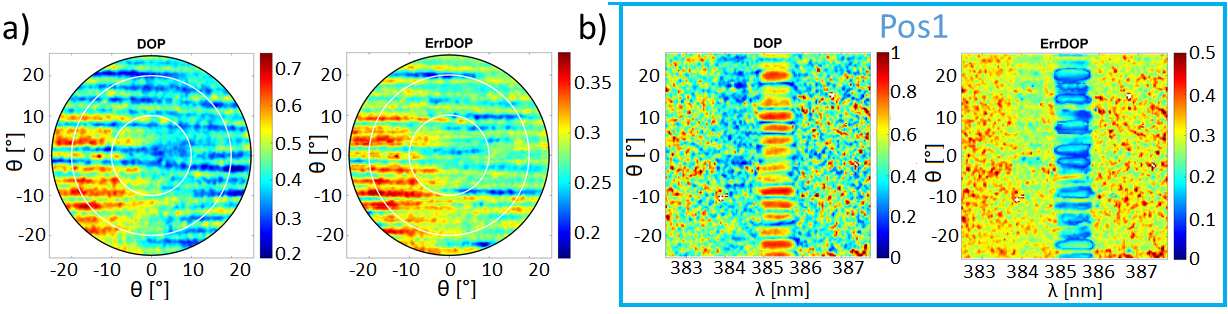
\includegraphics[width=1\textwidth]{Bilder/MgO/DOP_MgO_S2_0}
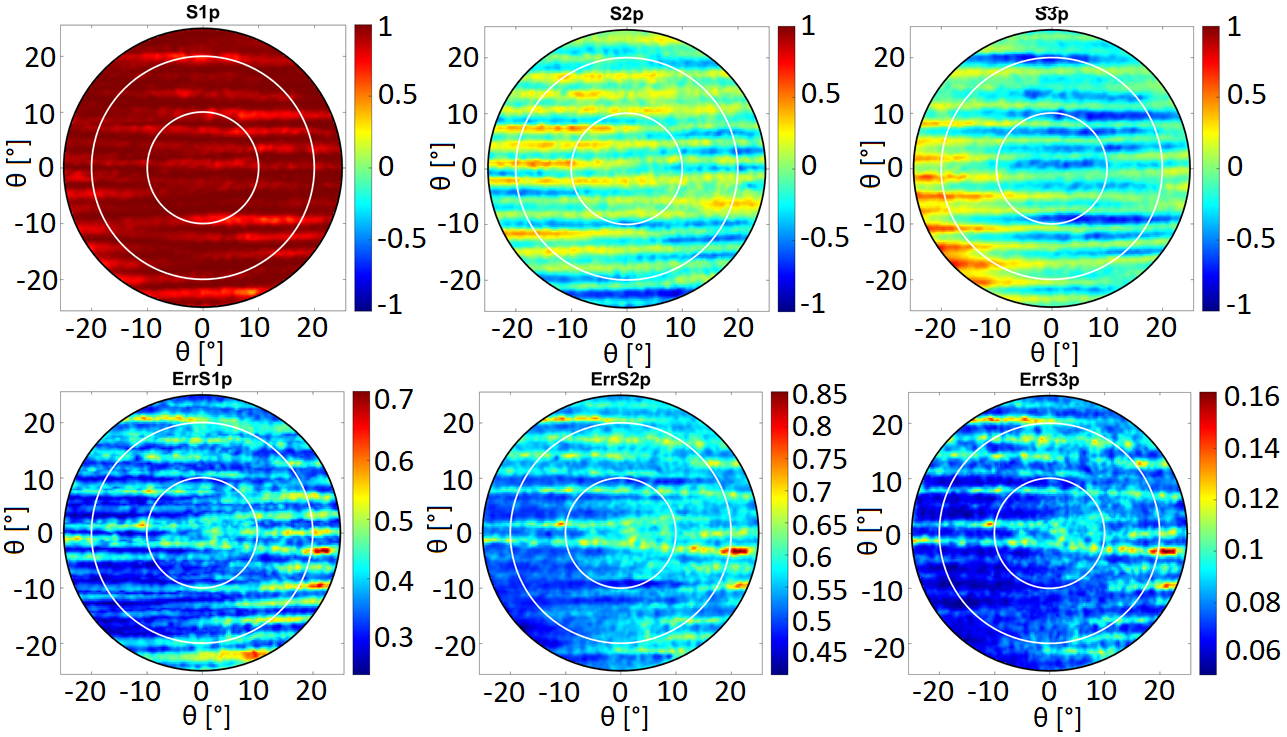
\includegraphics[width=0.75\textwidth]{Bilder/MgO/StokesP_S2_MgO_0}
\caption{Obere
\label{StokesP_S2_MgO_0}
\autoref{StokesP_S2_MgO_0}
\autoref{SpecP1_StokesP_Line_S2_MgO_0}
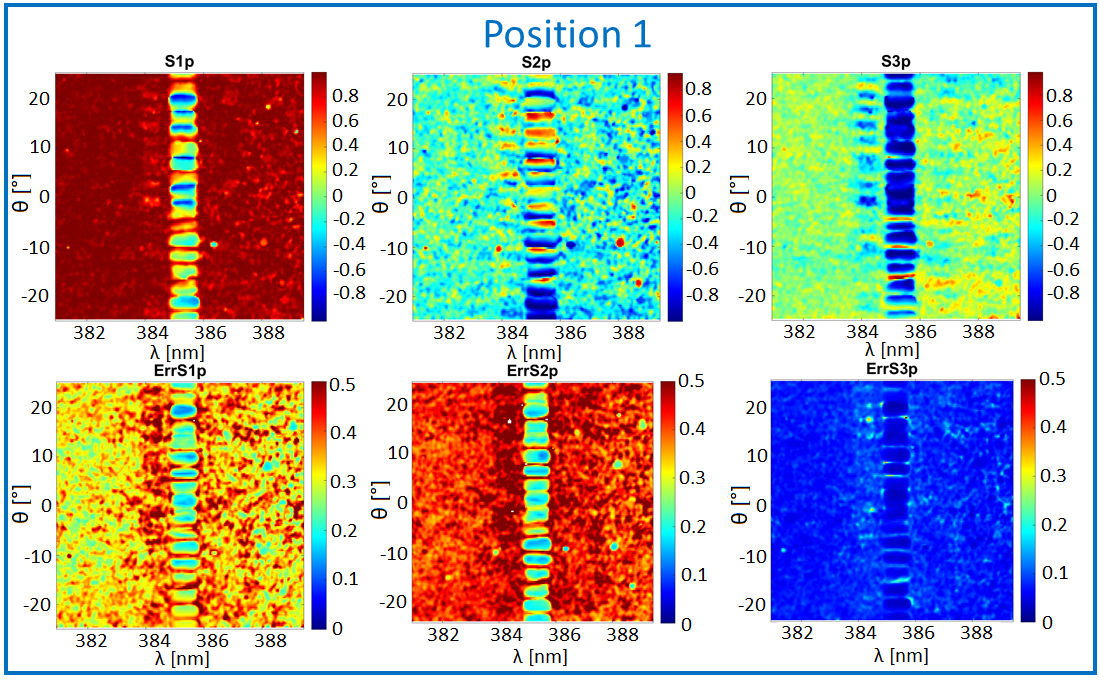
\includegraphics[width=0.8\textwidth]{Bilder/MgO/SpecP1_StokesP_S2_MgO_0}
\caption{Obere
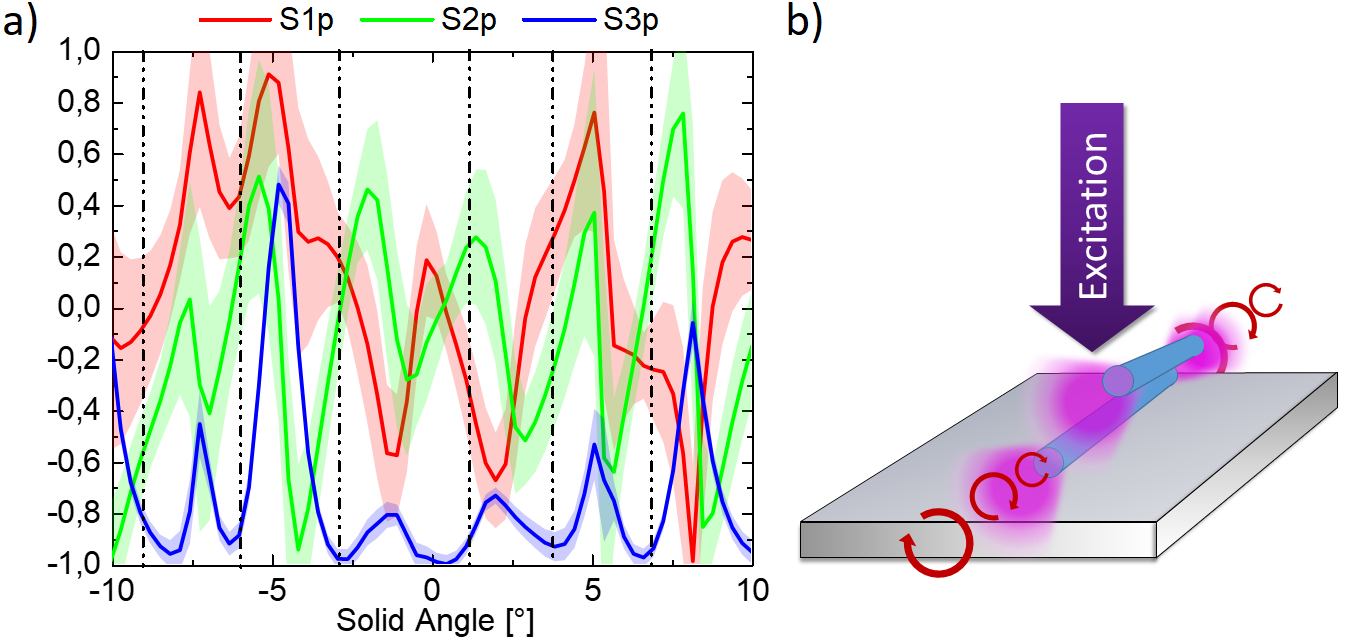
\includegraphics[width=.6\textwidth]{Bilder/MgO/SpecP1_StokesP_Line_S2_MgO_0}
\caption{a)
\autoref{S0_S2_MgO_0}
\end{figure}
\autoref{Sim})
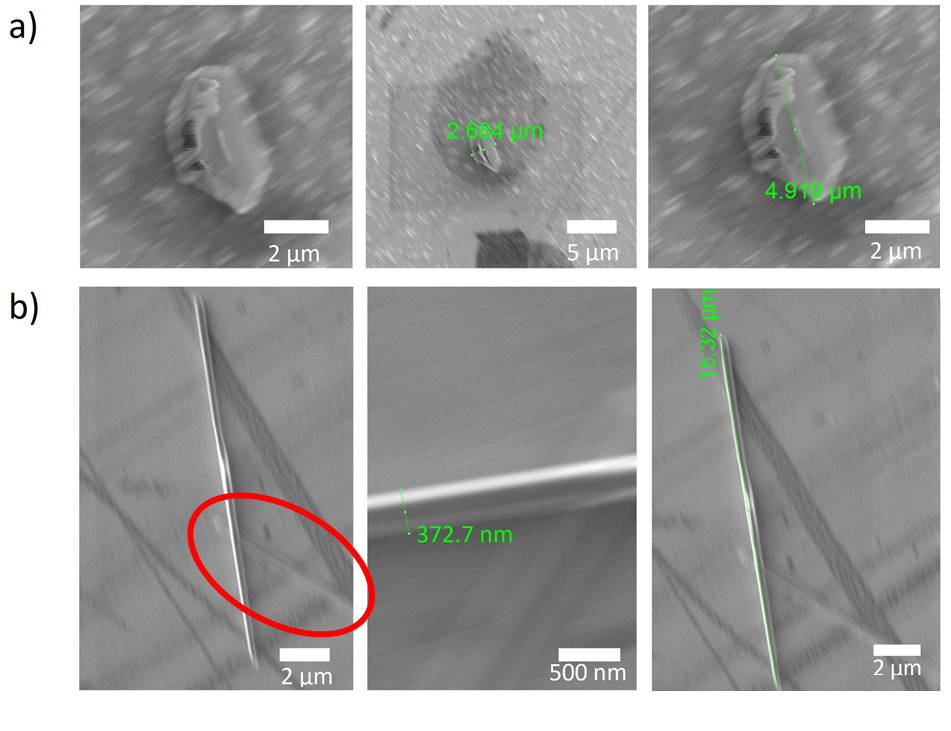
\includegraphics[width=.66\textwidth]{Bilder/Mag/SEM_Mag1}
\text{386.06
\textit{Whispering-Gallery-Moden}.
\autoref{Spectr_Mag}
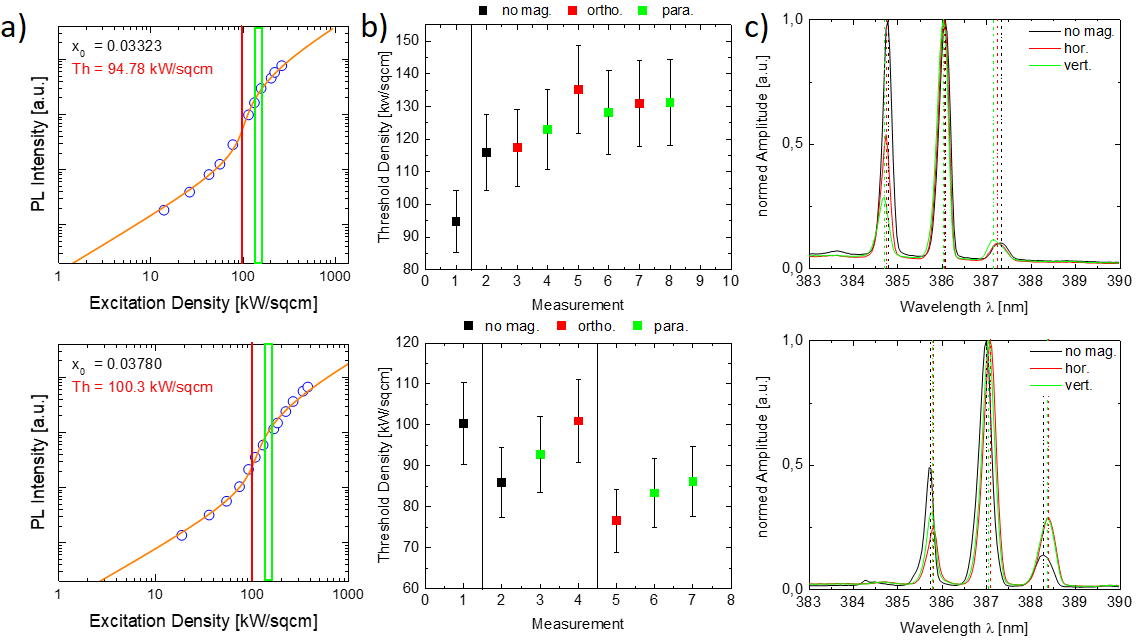
\includegraphics[width=1\textwidth]{Bilder/Mag/Spectr_Mag}
\autoref{SEM_Mag}
\centering
\caption{Fourierbilder
\autoref{DOP_Spec_Mag}
\autoref{DOP_Mag}
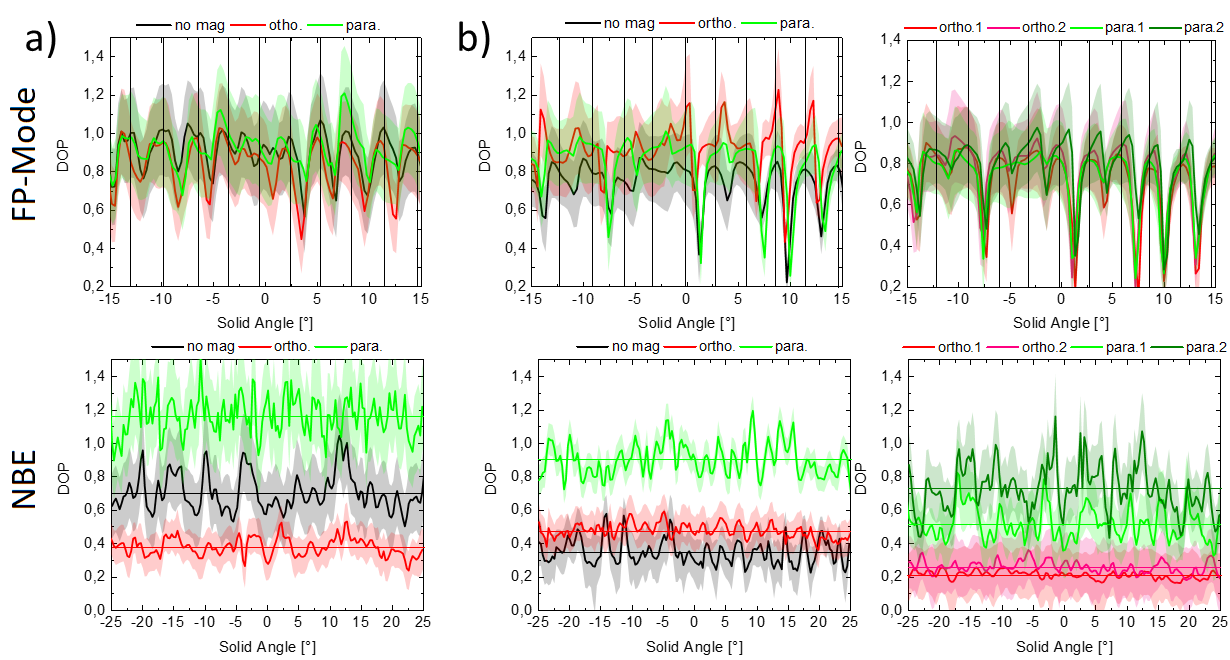
\includegraphics[width=1\textwidth]{Bilder/Mag/DOP_Mag}
\mbox{$\uplambda=$
\label{DOP_Mag}
\autoref{DOP_Mag}
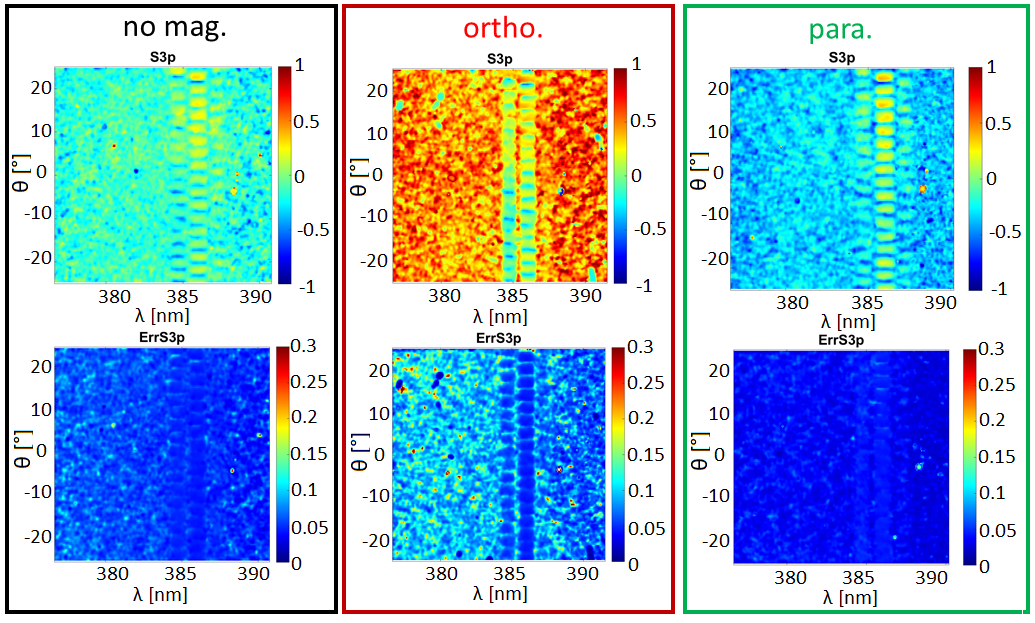
\includegraphics[width=.85\textwidth]{Bilder/Mag/Stokes_Spec_Mag}
\caption{Fourierbild
\centering
\autoref{Stokes_NBE_repeat},
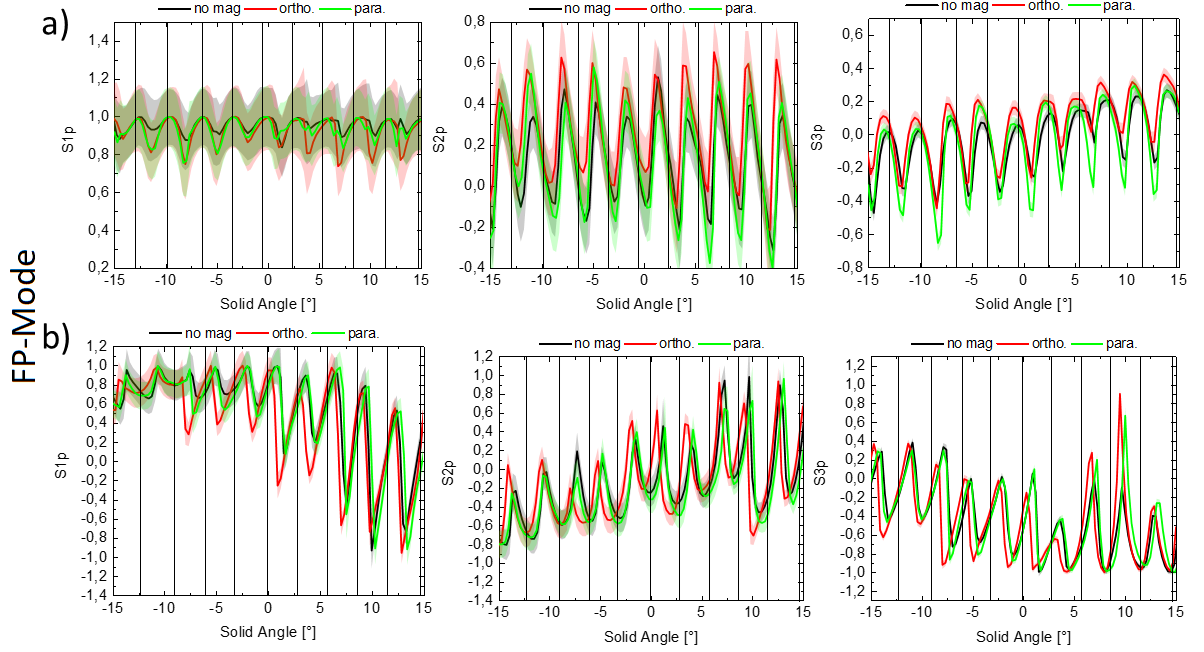
\includegraphics[width=1\textwidth]{Bilder/Mag/Stokes_Mag}
\includegraphics[width=1\textwidth]{Bilder/Mag/Stokes_NBE_Mag}
\caption{Gemittelte
\autoref{DPM})
\autoref{DPM_Mag}).\FloatBarrier
\centering
\caption{Wiederholte
